\chapter{Mathematical Analysis: Part I}

\begin{quote}
\emph{
We now embark on a great undertaking: building a rigorous framework for calculus. Our journey through logic and set theory has provided the tools; the ordered structures of Chapter 1 have revealed a critical insight—the rational numbers, though dense, are incomplete. They possess gaps, like the legendary irrational $\sqrt{2}$, which defy representation as a ratio.
}

\emph{
This chapter confronts that insufficiency. We will construct the real number system, a complete, continuous tapestry woven to fill these voids. Its cornerstone is the Completeness Axiom, which guarantees that bounded sets have precise bounds, a property the rationals fatally lack.
}

\emph{
Upon this unshakable foundation, we will erect the central pillars of analysis: the precise theory of limits, the formal definition of continuity, and the powerful machinery of the derivative and integral in the next chapter. This is the transition from intuitive calculation to profound understanding—from calculus to Analysis.
}
\end{quote}

\section{Extension of the Number System}
If asked about the foundation of mathematical analysis, the answer is clear: the axiom of real numbers. In this part, we will start from Peano Axioms to form the axioms of natural numbers. And for practical purposes, we extend it to integers and rational numbers. Then, to support theorems of calculus, we construct the axioms of real numbers and complex numbers.

Before we officially start this part, we need to clarify three simple principles:
\begin{description}
    \item[Motivation Principle (Solving a Limitation)] Each expansion is driven by the need to perform an operation that is not always possible within the smaller number system. The primary goal is to achieve \textbf{closure} under this new operation.
    \item[Embedding Principle (Preserving the Original Structure)] The smaller, original number system must be isomorphic to a subsystem of the new, larger number system. This is achieved by constructing an \textbf{injective embedding} that preserves all the essential operations (like addition and multiplication) and properties of the original system.
    \item[Minimality Principle (The "Smallest" Extension)] The new number system should be the "smallest" or "most economical" extension that satisfies the first two principles. It should introduce \emph{only} the elements necessary to solve the limitation, without any superfluous structure.
\end{description}

\subsection{Peano Axioms and Natural Numbers}
Peano axioms define natural numbers using 5 axioms:
\begin{definition}[Peano’s Axioms]
A set $\mathbb{N}$ is called the \textbf{natural number set} if it satisfies the following properties (with a "successor" function $S: \mathbb{N} \to \mathbb{N}$):
\begin{enumerate}
    \item $0 \in \mathbb{N}$. (Zero is a natural number.)
    \item $\forall a \in \mathbb{N} (S(a) \in \mathbb{N})$. (If $a$ is a natural number, the successor of $a$ is a natural number.)
    \item $\forall a \in \mathbb{N} (S(a) \ne 0)$. (Zero is not the successor of any natural number.)
    \item $\forall a, b \in \mathbb{N} (S(a) = S(b) \to a = b)$. (Two numbers whose successors are equal are themselves equal.)
    \item $\forall K \subseteq \mathbb{N} [(0 \in K \wedge \forall n (n \in K \to S(n) \in K)) \to K = \mathbb{N}]$. (If a set S of numbers contains zero and also the successor of every number in S, then every number is in S. This is the \textbf{Axiom of Induction}.)
\end{enumerate}
We denote the successor of $a$ as $a+1$.
\end{definition}

The definition of the natural numbers has a very strong relationship with the concept of mathematical induction and the well-ordered set. In fact, they are logically equivalent (assuming the other axioms).
\begin{itemize}
    \item Peano axioms ensure the validity of mathematical induction (Axiom 5 is MI).
    \item Peano axioms ensure the validity of the well-ordering principle.
\end{itemize}

Here, we will prove the logical equivalence of the well-ordering principle (WOP) and mathematical induction (MI).

\begin{proof}[MI implies Well-Ordering Principle]
\textbf{To prove:} every non-empty subset of natural numbers has a least element.
Assume, for contradiction, that there exists a non-empty subset $A \subseteq \mathbb{N}$ that has \emph{no} least element.
Define another set $B = \{ n \in \mathbb{N} \mid n < a \text{ for all } a \in A \}$. ($B$ is the set of all numbers strictly smaller than everything in $A$).

\textbf{Base Case:} $0 \in B$?
If $0 \notin B$, then there exists some $a \in A$ such that $0 \ge a$. Since $a \in \mathbb{N}$, this implies $a=0$. So $0 \in A$. Since 0 is the smallest natural number, it would be the least element of $A$, contradicting the assumption that $A$ has no least element. Thus, $0 \in B$.

\textbf{Inductive Step:} Assume $k \in B$ and prove $S(k) \in B$.
Inductive Hypothesis: $k \in B$, meaning $k < a$ for all $a \in A$.
If $S(k) \notin B$, then there exists some $a \in A$ such that $S(k) \ge a$.
From the hypothesis, $k < a$. Combined with $S(k) \ge a$, and since numbers are discrete, the only possibility is $a = S(k)$.
So $S(k) \in A$. Furthermore, since all numbers smaller than $S(k)$ (like $k$) are in $B$ (and thus not in $A$), $S(k)$ would be the least element of $A$.
This contradicts the assumption that $A$ has no least element. Therefore, $S(k) \in B$.

\textbf{Conclusion:} By the principle of Mathematical Induction (Axiom 5), $B = \mathbb{N}$.
Since $A$ is non-empty, take any element $a \in A$. Because $B = \mathbb{N}$, $a \in B$.
By the definition of $B$, this means $a < a$, which is a contradiction.
The initial assumption that $A$ has no least element must be false.
Therefore, every non-empty subset of $\mathbb{N}$ has a least element.
\end{proof}

\begin{proof}[Well-Ordering Principle implies MI]
(This part is left for the readers to practice.)
\end{proof}

\subsubsection*{Cardinality}
The concept “amount” is clear for finite sets. But for an infinite set, how can we measure the “size” of the set?
\begin{definition}[Cardinality / Equinumerosity]
Cardinality is an intrinsic property of sets. Two sets $A$ and $B$ are said to be \textbf{equinumerous} or have the same \textbf{cardinality}, denoted $A \approx B$ or $|A|=|B|$, if there exists a bijection $f: A \to B$.
\end{definition}

\begin{definition}
For two sets $A$ and $B$, if we can find an injection $f: A \to B$ but no bijection, we said the set $A$ is strictly smaller than set $B$, denoted $A \prec B$ or $|A| < |B|$. If there is an injection $f: A \to B$, we write $A \preceq B$ or $|A| \le |B|$.
\end{definition}

\begin{theorem}[Schröder-Bernstein Theorem]
If $A \preceq B$ and $B \preceq A$, then $A \approx B$.
\end{theorem}

\begin{definition}[Countable Set]
A set is \textbf{countable} if either it is finite or it can be made in one-to-one correspondence with the set of natural numbers $\mathbb{N}$. If a set is countably infinite, we define its cardinality as $\aleph_0$ (aleph-nought).
\end{definition}

\begin{theorem}[Cantor's Theorem]
For every non-empty set $A$, $A \prec \mathcal{P}(A)$. (That is, $|A| < |\mathcal{P}(A)|$).
\end{theorem}
(This implies there is no "largest" infinity.)

In section 2.3, we will know that the cardinality of the real number set $\mathbb{R}$ is $|\mathbb{R}| = |\mathcal{P}(\mathbb{N})| = 2^{\aleph_0}$, which is called the \textbf{Continuum}.

\paragraph{The Continuum Hypothesis (CH)}
Some students might be interested whether there exists any size of a set between $\aleph_0$ and $2^{\aleph_0}$. The Continuum Hypothesis (CH) is a famous conjecture that proposes there is no set $S$ such that $\aleph_0 < |S| < 2^{\aleph_0}$.

So can we determine whether it’s true or false? It was proven (by Kurt Gödel and Paul Cohen) that CH is "undecidable" within the standard ZFC foundation of mathematics. This means it can neither be proven true nor false using the accepted axioms, revealing a fundamental limitation of that system.

\subsection{Integers and Rational Numbers}
Why do we need integers and rational numbers? Why are natural numbers not enough?
\begin{definition}[Closure of operation]
Closure of operation refers to the property that when an operation is performed on members of a set, the result is always a member of the same set.
\end{definition}
In the set of natural numbers $\mathbb{N}$, operations like addition and multiplication are closed. But for subtraction ($3 - 5 = ?$) and division ($3 / 5 = ?$), $\mathbb{N}$ itself is not enough. Thus, we need to extend the number system.

\paragraph{Construction of Integers ($\mathbb{Z}$)}
\begin{definition}
The relation $R$ on $\mathbb{N} \times \mathbb{N}$ is defined as:
$$ (a,b) R (c,d) \iff a+d = b+c $$
(This is the formal way of saying $a-b = c-d$).
\end{definition}

\begin{theorem}
The relation $R$ is an equivalence relation on $\mathbb{N} \times \mathbb{N}$.
\end{theorem}
\begin{proof}
(Left for readers to practice: check reflexivity, symmetry, transitivity.)
\end{proof}

\begin{definition}[Integers $\mathbb{Z}$]
The \textbf{integers}, denoted as $\mathbb{Z}$, is the set of equivalence classes of $\mathbb{N} \times \mathbb{N}$ w.r.t the equivalence relation $R$. We denote the equivalence class $[(a,b)]$ as $a-b$.
\end{definition}

We can now define operations on $\mathbb{Z}$:
\begin{definition}[Operations on $\mathbb{Z}$]
\begin{itemize}
    \item \textbf{Addition:} $[(a,b)] + [(c,d)] = [(a+c, b+d)]$
    \item \textbf{Negation:} $-[(a,b)] = [(b,a)]$
    \item \textbf{Subtraction:} $[(a,b)] - [(c,d)] = [(a,b)] + (-[(c,d)]) = [(a,b)] + [(d,c)] = [(a+d, b+c)]$
\end{itemize}
\end{definition}
Because $a,b,c,d \in \mathbb{N}$, and $\mathbb{N}$ is closed under addition, $a+d$ and $b+c$ also belong to $\mathbb{N}$. This means that subtraction is closed for integers. The construction of $\mathbb{Z}$ from $\mathbb{N}$ via ordered pairs is a perfect example of the principles of number system expansion.

\paragraph{Construction of Rational Numbers ($\mathbb{Q}$)}
Though $\mathbb{Z}$ is closed under subtraction, it is not closed under division. That’s why we still need to extend from integers to rational numbers.

\begin{definition}
Let $\mathbb{Z}^* = \mathbb{Z} - \{0\}$. The relation $R$ on $\mathbb{Z} \times \mathbb{Z}^*$ is defined by:
$$ (a,b) R (c,d) \iff ad = bc $$
(This is the formal way of saying $a/b = c/d$).
\end{definition}
It’s clear that this relation $R$ is an equivalence relation.

\begin{definition}[Rational Numbers $\mathbb{Q}$]
The set of \textbf{rational numbers}, denoted $\mathbb{Q}$, is the set of equivalence classes of $\mathbb{Z} \times \mathbb{Z}^*$ w.r.t the equivalence relation $R$. We denote the class $[(a,b)]$ as $a/b$.
\end{definition}

\paragraph{Density of Rational Numbers}
There is a very different property of rational numbers compared to integers. The rational number set is a \textbf{dense order set}. We can’t always find an intermediate number between two integers (e.g., 1 and 2), but we can always find a rational intermediate value between two rational numbers.
\begin{proof}
For two rational numbers $a$ and $b$ with $a < b$, their average $m = (a+b)/2$ is also a rational number, and $a < m < b$. Thus, we found an intermediate number between them.
\end{proof}
This property (the density of $\mathbb{Q}$ in $\mathbb{R}$) is essential for constructing and understanding the real number system. In topology, $\mathbb{Q}$ is a countable dense subset of $\mathbb{R}$, making $\mathbb{R}$ a separable space.

\subsection{Real Numbers and Complex Numbers}
The rational numbers $\mathbb{Q}$, while dense, are not \emph{complete}. They contain "gaps". For example, the set $A = \{ x \in \mathbb{Q} \mid x^2 < 2 \}$ has upper bounds in $\mathbb{Q}$ (e.g., 1.5), but it has no \emph{least} upper bound \emph{within} $\mathbb{Q}$. The "number" $\sqrt{2}$ is missing. We construct the real numbers $\mathbb{R}$ to fill these gaps.

\subsubsection{Construction of Real Numbers by Dedekind Cuts}

\begin{definition}[Dedekind Cut]
A \textbf{Dedekind cut} is a pair $(A, B)$ of subsets of $\mathbb{Q}$ satisfying:
\begin{enumerate}
    \item $A$ and $B$ are non-empty and form a partition of $\mathbb{Q}$ (i.e., $A \cup B = \mathbb{Q}$ and $A \cap B = \emptyset$).
    \item Every element of $A$ is less than every element of $B$.
    \item $A$ has no greatest element.
\end{enumerate}
The set $A$ is called the \textbf{lower class} and $B$ the \textbf{upper class}. A real number is defined as a Dedekind cut.
\end{definition}

For example, the real number $\sqrt{2}$ is represented by the cut where:
\begin{itemize}
    \item $A = \{x \in \mathbb{Q} \mid x < 0 \text{ or } x^2 < 2\}$
    \item $B = \{x \in \mathbb{Q} \mid x > 0 \text{ and } x^2 > 2\}$
\end{itemize}

\begin{definition}[Order on Real Numbers]
For two real numbers $\alpha = (A_1, B_1)$ and $\beta = (A_2, B_2)$, we define $\alpha < \beta$ if $A_1 \subset A_2$ (proper subset). We define $\alpha = \beta$ if $A_1 = A_2$.
\end{definition}

\begin{definition}[Addition of Real Numbers]
Let $\alpha = (A_1, B_1)$ and $\beta = (A_2, B_2)$ be real numbers. Define:
\begin{itemize}
    \item $A = \{a_1 + a_2 \mid a_1 \in A_1, a_2 \in A_2\}$
    \item $B = \mathbb{Q} \setminus A$
\end{itemize}
Then $\alpha + \beta$ is defined as the cut $(A, B)$.
\end{definition}

\begin{definition}[Multiplication of Positive Real Numbers]
For positive real numbers $\alpha = (A_1, B_1)$ and $\beta = (A_2, B_2)$ (where "positive" means they contain some positive rationals in their lower classes), define:
\begin{itemize}
    \item $A = \{a_1a_2 \mid a_1 \in A_1, a_2 \in A_2, a_1 > 0, a_2 > 0\} \cup \{q \in \mathbb{Q} \mid q \le 0\}$
    \item $B = \mathbb{Q} \setminus A$
\end{itemize}
Then $\alpha \cdot \beta$ is defined as the cut $(A, B)$. For other sign combinations, we adjust the definition accordingly.
\end{definition}

\begin{definition}[Additive Inverse]
For a real number $\alpha = (A, B)$, define its additive inverse $-\alpha$ by:
\begin{itemize}
    \item $A' = \{-b \mid b \in B, b \text{ is not the smallest element of } B\}$
    \item $B' = \mathbb{Q} \setminus A'$
\end{itemize}
Then $-\alpha = (A', B')$.
\end{definition}

These operations make $\mathbb{R}$ an ordered field. The multiplicative inverse can be defined similarly for non-zero elements.

Now we can define the fundamental concepts of analysis:

\begin{definition}[Upper Bound]
Let $S \subseteq \mathbb{R}$. A number $u$ is an \textbf{upper bound} of $S$ if $s \le u$ for all $s \in S$. A number $l$ is a \textbf{lower bound} of $S$ if $l \le s$ for all $s \in S$.
\end{definition}

\begin{definition}[Supremum]
The \textbf{supremum} (or \textbf{least upper bound}) of $S$, denoted $\sup S$, is the smallest upper bound of $S$. That is:
\begin{enumerate}
    \item $s \le \sup S$ for all $s \in S$. ($\sup S$ is an upper bound.)
    \item If $v$ is any upper bound of $S$, then $\sup S \le v$. (It is the \emph{least} upper bound.)
\end{enumerate}
The definition of \textbf{infimum} (or \textbf{greatest lower bound}), denoted $\inf S$, is similar.
\end{definition}

\begin{theorem}[Completeness Axiom]
Every non-empty subset of $\mathbb{R}$ that is bounded above has a supremum in $\mathbb{R}$.
\end{theorem}
(The case for the infimum is analogous: every non-empty subset of $\mathbb{R}$ that is bounded below has an infimum in $\mathbb{R}$.)

\begin{proof}
In the Dedekind cut construction, the supremum of a bounded set $S$ of real numbers is given by the union of the lower classes of all elements in $S$. More precisely, if $S = \{\alpha_i = (A_i, B_i)\}$ is bounded above, then:
\[
\sup S = \left(\bigcup_i A_i, \mathbb{Q} \setminus \bigcup_i A_i\right)
\]
This pair forms a Dedekind cut and satisfies the definition of supremum.
\end{proof}

The completeness axiom is fundamental to analysis and distinguishes $\mathbb{R}$ from $\mathbb{Q}$. It ensures that limits of Cauchy sequences exist, continuous functions attain their maximum and minimum on closed intervals, and many other essential properties.

\begin{definition}[Archimedean Property]
The real numbers satisfy the \textbf{Archimedean property}: for any $x \in \mathbb{R}$, there exists a natural number $n$ such that $n > x$. Equivalently, for any $\epsilon > 0$, there exists $n \in \mathbb{N}$ such that $1/n < \epsilon$.
\end{definition}

\begin{theorem}[Density of Rationals]
Between any two distinct real numbers, there exists a rational number. That is, $\mathbb{Q}$ is \textbf{dense} in $\mathbb{R}$.
\end{theorem}

While $\mathbb{R}$ solves the completeness problem of $\mathbb{Q}$, it is not \textbf{algebraically closed}. There are polynomial equations with real coefficients that have no real solutions, such as $x^2 + 1 = 0$. This motivates the extension to complex numbers.

\begin{definition}[Complex Numbers]
The set of \textbf{complex numbers}, denoted $\mathbb{C}$, consists of all expressions of the form $a + bi$, where $a, b \in \mathbb{R}$ and $i$ is the \textbf{imaginary unit} satisfying $i^2 = -1$. For $z = a + bi \in \mathbb{C}$:
\begin{itemize}
    \item $a$ is called the \textbf{real part}, denoted $\Re(z)$
    \item $b$ is called the \textbf{imaginary part}, denoted $\Im(z)$
\end{itemize}
\end{definition}

Two complex numbers $a + bi$ and $c + di$ are equal if and only if $a = c$ and $b = d$.

\begin{definition}[Operations on Complex Numbers]
For complex numbers $z = a + bi$ and $w = c + di$, we define:
\begin{itemize}
    \item \textbf{Addition}: $z + w = (a + c) + (b + d)i$
    \item \textbf{Multiplication}: $zw = (ac - bd) + (ad + bc)i$
\end{itemize}
\end{definition}

With these operations, $\mathbb{C}$ forms a field. The real numbers $\mathbb{R}$ can be identified with the subset $\{a + 0i : a \in \mathbb{R}\}$ of $\mathbb{C}$.

\begin{definition}[Complex Conjugate and Modulus]
For $z = a + bi \in \mathbb{C}$:
\begin{itemize}
    \item The \textbf{complex conjugate} is $\bar{z} = a - bi$
    \item The \textbf{modulus} (or absolute value) is $|z| = \sqrt{a^2 + b^2}$
\end{itemize}
\end{definition}

\begin{theorem}[Properties of Conjugate and Modulus]
For $z, w \in \mathbb{C}$:
\begin{enumerate}
    \item $\overline{z + w} = \bar{z} + \bar{w}$
    \item $\overline{zw} = \bar{z} \cdot \bar{w}$
    \item $z\bar{z} = |z|^2$
    \item $|zw| = |z||w|$
    \item $|z + w| \le |z| + |w|$ (Triangle Inequality)
\end{enumerate}
\end{theorem}

\begin{theorem}[Fundamental Theorem of Algebra]
Every non-constant polynomial with complex coefficients has at least one complex root. Equivalently, $\mathbb{C}$ is algebraically closed.
\end{theorem}

This theorem is profound: while we extended $\mathbb{R}$ to $\mathbb{C}$ to solve the equation $x^2 + 1 = 0$, we actually obtained a number system where every polynomial equation has a solution.

\begin{definition}[Polar Form of Complex Numbers]
Any complex number $z = a + bi \neq 0$ can be written in \textbf{polar form} as:
\[
z = r(\cos\theta + i\sin\theta)
\]
where $r = |z| > 0$ is the modulus and $\theta$ is the \textbf{argument} of $z$, satisfying $\tan\theta = b/a$.
\end{definition}

Using Euler's formula $e^{i\theta} = \cos\theta + i\sin\theta$, we can write $z = re^{i\theta}$.

\begin{theorem}[De Moivre's Theorem]
For any integer $n$ and complex number $z = r(\cos\theta + i\sin\theta)$:
\[
z^n = r^n(\cos(n\theta) + i\sin(n\theta))
\]
\end{theorem}

This theorem simplifies computations with powers and roots of complex numbers.

The complex numbers provide a powerful framework for many areas of mathematics, physics, and engineering. They allow us to:
\begin{itemize}
    \item Solve all polynomial equations
    \item Represent periodic phenomena using complex exponentials
    \item Analyze signals and systems in electrical engineering
    \item Study fluid dynamics and electromagnetism
    \item Develop the mathematical foundation of quantum mechanics
\end{itemize}

\section{Sequence Limit and The Properties of Real Numbers}

As long as we finished the content about real numbers, we will now move on to the the core of the mathematical analysis: the \textbf{limit}. Why I claim that the limit is the core concept of mathematical analysis? In the following content you will realize that almost all the concept has some kind of connection with limit. I can say that the limit is the basis of many theory. And the language of limit represents a dynamic, approaching, and rigorous mathematical mindset. Let us begin.

\subsection{Definitions and Basic Properties}

\subsubsection{The Definition of Limits}

\begin{definition}[limit of a sequence]
A sequence $\{a_n\}$ converges to a real number $A$ if for all $\epsilon > 0$, there exists an integer $N$ such that $|a_n - A|<\epsilon$ if $n\ge N$. The number $A$ is the limit of the sequence and we write:
\[\lim_{n \to \infty} a_n = A\]
\end{definition}
Naively speaking, if the sequence $\{a_n\}$ is a \textbf{convergent sequence} and $A$ is the limit of the sequence, the value of $a_n$ become arbitrarily close to a finite number $A$. You can get any value that is anyhow closer to the convergence $A$, once you pick a big enough $n$.

In a more commonly used language, if we pick an open interval in the real number line, whose center is $a$ and radius is $\epsilon$, written as $(a-\epsilon,a+\epsilon)$. We call this kind of intervals the neighborhood, denoted as $O(a,\epsilon)$:

\[O(a,\epsilon)=\{x|a-\epsilon < x < a+\epsilon\}\]
And what the definition said is that for all terms after $a_n$ fall within the $O(a,\epsilon)$. Since the neighborhood is contractive, the sequence eventually converges to $a$.

However, in the contrary, if a sequence $\{a_n\}$ is not convergent, we say it is a \textbf{divergent sequence}. Rigorously speaking, if for all $\epsilon > 0$, $N \in \mathbb{N}^*$ and $A \in \mathbb{R}$, there exists at least one $n_0$, $|a_{n_0} - A| > \epsilon$.

For those sequences converges to $0$, we call those sequences \textbf{infinitesimal}. 

\begin{remark}
When we talk about infinitesimal, what we are discussing about is a sequence rather than a simple number. Be clear that infinitesimal is not a number.
\end{remark}

\subsubsection{Properties of Limits}

After we define what is limit, let's take a look at it's properties.

\begin{theorem}[the uniqueness of limit]
The limit of a convergent sequence must be unique.
\end{theorem}
\begin{proof}
Assume there exists a sequence $\{a_n\}$ that converges to two different values $a$ and $b$, $a\neq b$. According to the definition of limit:

\[
\forall\epsilon>0, \exists N_1, n>N_1:|x_n - a|< \epsilon/2
\]
\[
\forall\epsilon>0, \exists N_2, n>N_2:|x_n - b|< \epsilon/2
\]
Pick $N=max\{N_1,N_2\}$, according to the triangle inequality, then $\forall n>N$ we have:

\[
|a-b| = |a-x_n+x_n-b| \leq |x_n-a|+|x_n-b|<\epsilon
\]
Since $\epsilon$ can get arbitrarily close to $0$, we know that $a=b$ 
\end{proof}

\begin{theorem}
A convergent sequence must be bounded.
\end{theorem}
\begin{remark}
However, the contrapositive is not always true. A bounded sequence may not be convergent.

Consider $a_n = (-1)^n$, the sequence $\{a_n\}$ bounded from $-1$ to $1$, but the sequence won't converges to any value.

In the future may be we can add a stronger condition to make the $\{a_n\}$ convergent. If you are interested, please move on to the content in 2.2.2.
\end{remark}

\begin{proof}
Assume $\{a_n\}$ is a convergent sequence, the limit is $a$. According to the definition of limit, we pick $\epsilon = 1$, thus $\exists N, \forall n > N:|x_n-a|<1$, then $a-1<x_n<a+1$

let $m = max\{a_1, a_2, ..., a_N, a+1\}$, $M = min\{a_1, a_2, ..., a_N, a-1\}$

Then we have $m \leq x_n \leq M$, which means that the sequence $\{x_n\}$ is bounded.
\end{proof}

\begin{theorem}[isotonicity]
Assume we have two sequence $\{x_n\}$ and $\{y_n\}$, they converges to two different limits $a$ and $b$, and $a<b$. There exists a $N$, $\forall n>N$, $x_n<y_n$
\end{theorem}

\begin{proof}
For two sequence $\{x_n\}$ and $\{y_n\}$ that converge to two different values $a$ and $b$. Let's assume $a>b$

According to the definition of limit, we take $\epsilon = \frac{a-b}{2}$, and we have:

\[
\exists N_1, \forall n>N_1, |x_n-a| < \epsilon
\]

\[
\exists N_2, \forall n>N_2, |y_n-b| < \epsilon
\]
Thus we have: $x_n > (a+b)/2 >y_n$ , pick $N = max \{N_1,N_2\}$, then we have $\forall n > N, x_n>y_n$. Finally we can claim that the limits have the property of isotonicity.
\end{proof}

\newpage

\begin{theorem}[the calculations' law of limits]

Assume that there exist two limits:

\[\lim_{n \to \infty} x_n = a, \lim_{n \to \infty} y_n = b\]
And we have:
\begin{itemize}
    \item $\lim_{n \to \infty} (\alpha x_n + \beta y_n) = \alpha a + \beta b$, for two constants $\alpha$ and $\beta$.
    \item $\lim_{n \to \infty} x_ny_n = ab$
    \item $\lim_{n \to \infty} (\frac{x_n}{y_n}) = \frac{a}{b},(b\neq0)$
\end{itemize}
\end{theorem}
We recommend the readers finish the proof above themselves.

After we finished the definition and some basic properties of the convergent sequence, we will now move on to define a kind of not-convergent sequence: \textbf{the infinity}.

\subsubsection{Infinity}

\begin{definition}[Infinity]
If we have a sequence $\{x_n\}$, for every given $G$, $G>0$, we can find $N \in \mathbb{N}$, $\forall n > N$, we have $|x_n|>G$, we call the sequence $\{x_n\}$ is a infinity, denoted as:

\[\lim_{n \to \infty} x_n = \infty\]

\end{definition}

Just like infinitesimal, infinity is also a sequence rather that a number. But in some conditions, we will deal with it as if it is a number.

If a infinity start to be positive from some point, we call this form of infinity the \textbf{positive infinity}. We can define what is negative infinity likewise. We denote them specially like this:

\[
\lim_{n \to \infty} a_n = + \infty,(\lim_{n \to \infty} a_n = - \infty)
\]

\begin{theorem}
The infinity has special relationship with the infinitesimal:
The sequence $\{x_n\}(x_n \neq 0)$ is infinity iff $\{\frac{1}{x_n}\}$ is infinitesimal. 
\end{theorem}

Using the definition of the limit will be enough to prove this theorem. We'll skip this part here.

\begin{theorem}
Assume $\{x_n\}$ is a infinity, if when $n>N_0$, $|y_n| \ge \delta >0$, then $\{x_n y_n\}$ is infinity.
\end{theorem}

\begin{inference}
Assume $\{x_n\}$ is infinity, $\lim_{n \to \infty} y_n = b \neq 0$, then $\{x_n y_n\}$ and $\{\frac{x_n}{y_n}\}$ are both infinity.
\end{inference}

\subsubsection{Stolz Theorem}

With the help of the definitions of the limit, we can calculate various kinds of limits using algebraic techniques and the definition of limit. But when we face certain forms of limit like $\frac{0}{0}$ and $\frac{\infty}{\infty}$, they are especially tricky to deal with. But with the help of \textbf{Stolz theorem} we are going to introduced now, it will be much easier to deal with them (in some occasions).

\begin{definition}[Increasing Function]
If a sequence $\{x_n\}$ satisfies: $x_n \leq x_{n+1}, n=1,2,3\cdots$, we will call it \textbf{the monotone increasing function}.
\end{definition}

\begin{definition}[Strict Monotone Increasing Function]
If a sequence $\{x_n\}$ satisfies: $x_n < x_{n+1}, n=1,2,3\cdots$, we will call it the \textbf{strict monotone increasing function}.
\end{definition}

\begin{theorem}
Let $\{y_n\}$ be a \textbf{strict monotone increasing positive infinity}, and:
\[
\lim_{n \to \infty} \frac{x_n -x_{n-1}}{y_n-y_{n-1}}=a
\]

Then we have that:
\[\lim_{n \to \infty}\frac{x_n}{y_n}=a\]

\end{theorem}

\begin{proof}
Let's consider the condition when $a=0$.
Because $\lim_{n \to \infty} \frac{x_n -x_{n-1}}{y_n-y_{n-1}}=0$, according to the definition of limit, we know that:

\[
\forall\epsilon > 0, \exists N_1,\forall n> N_1:|x_n-x_{n-1}|<\epsilon(y_n-y_{n-1})
\]

Because $\{y_n\}$ is infinity, we can let $y_{N_1} > 0$ obviously. For the inequality above, we take everything from $N_1$ to $n$, and then we add them together, we have:

\[
|x_n-x_{N_1}|\leq |x_n-x_{n-1}| +|x_{n-1}-x_{n-2}|+\cdots+ |x_{N_1+1}-X_{N_1}|
\]

\[
 < \epsilon (y_n-y_{n-1}) + \cdots + \epsilon (y_{N_1+1}-y_{N_1}) = \epsilon (y_n-y_{n-1})
\]
Divide both side of the inequality by $y_n$, and we have:
\[
|\frac{x_n}{y_n}-\frac{x_{N_1}}{y_n}|\leq \epsilon (1-\frac{y_{N_1}}{y_n}) \leq \epsilon
\]
And, for a fixed $N_1$, we can pick $N>N_1$, $\forall n >N: |\frac{x_{N_1}}{y_n}|<\epsilon$, then we have:

\[
|\frac{x_n}{y_n}|<\epsilon+|\frac{x_{N_1}}{y_n}|<2\epsilon
\]

For other conditions: if $a$ is a bounded value, and $a \neq 0$, let ${x_n}'=x_n-ay_n$, and with the help of the proof above, we can reach the conclusion.

When $a=+\infty$, We take the reciprocal of $\frac{x_n}{y_n}$. Similarly, it is not difficult to reach a conclusion.

\end{proof}


\subsection{Convergence Criteria and the Properties of the Real Number System}

Before we discuss more advanced concepts in analysis (such as derivatives and integrals), we must first firmly establish a fundamental property of the real number system $\mathbb{R}$: \textbf{Completeness}. It is this property that distinguishes the real numbers $\mathbb{R}$ from the rational numbers $\mathbb{Q}$ and serves as the bedrock for all important theorems in analysis.

\subsubsection{The Completeness of the Real Number System}

The completeness of the real number system can be expressed in several equivalent ways. Let's take a review. (The proof is in section 2.1.3)

\begin{theorem}[The Completeness Axiom]
\label{thm:completeness_en}
Every non-empty subset of $\mathbb{R}$ that is bounded above has a supremum in $\mathbb{R}$.
\end{theorem}

This axiom, while seemingly simple, directly leads to the first major convergence criterion in analysis.

\subsubsection{The Monotone Convergence Theorem}

We previously defined monotone increasing sequences. The Completeness Axiom guarantees that a bounded monotone sequence must converge.

\begin{theorem}[Monotone Convergence Theorem]
\label{thm:mct_en}
A monotone sequence (either increasing or decreasing) that is bounded must converge.
\begin{itemize}
    \item (i) If $\{x_n\}$ is a monotone increasing and bounded above, then $\lim_{n \to \infty} x_n = \sup \{x_n\}$.
    \item (ii) If $\{x_n\}$ is a monotone decreasing and bounded below, then $\lim_{n \to \infty} x_n = \inf \{x_n\}$.
\end{itemize}
\end{theorem}

\begin{proof}
We will prove (i); the proof for (ii) is analogous.
Let $\{x_n\}$ be a monotone increasing sequence that is bounded above. Let $S = \{x_n \mid n \in \mathbb{N}\}$ be the set of its terms.
By hypothesis, $S$ is non-empty and bounded above.
By the Completeness Axiom, $S$ must have a supremum. Let $a = \sup S$.

We will now prove that $\lim_{n \to \infty} x_n = a$.
According to the definition of a limit, we must show:
\[
\forall \epsilon > 0, \exists N \in \mathbb{N}, \forall n > N: |x_n - a| < \epsilon
\]
This is equivalent to $a - \epsilon < x_n < a + \epsilon$.

\begin{enumerate}
    \item First, by the definition of a supremum, $a$ is an upper bound for $S$, so $x_n \leq a$ for all $n$. It is clear that $x_n < a + \epsilon$.
    \item Next, consider $a - \epsilon$. By the definition of a supremum, $a$ is the \textit{least} upper bound, which means $a - \epsilon$ (being smaller than $a$) \textit{cannot} be an upper bound for $S$.
    \item Since $a - \epsilon$ is not an upper bound, there must exist some element $x_N$ in $S$ such that $x_N > a - \epsilon$.
    \item Because $\{x_n\}$ is monotone increasing, for any $n > N$, we have $x_n \geq x_N$.
    \item Combining (1), (3), and (4), we have:
    \[
    \forall n > N: a - \epsilon < x_N \leq x_n \leq a < a + \epsilon
    \]
    This implies $\forall n > N: |x_n - a| < \epsilon$.
\end{enumerate}
Therefore, $\lim_{n \to \infty} x_n = a$.
\end{proof}

\subsubsection{The Cauchy Convergence Criterion}

The Monotone Convergence Theorem is powerful, but it requires the sequence to be monotone. For the general case, we need a criterion for convergence that does not depend on monotonicity, nor on knowing the value of the limit beforehand. This is the Cauchy Criterion.

\begin{definition}[Cauchy Sequence]
A sequence $\{x_n\}$ is called a \textbf{Cauchy Sequence} if:
\[
\forall \epsilon > 0, \exists N \in \mathbb{N}, \forall m, n > N: |x_m - x_n| < \epsilon
\]
Intuitively, a Cauchy sequence is one whose terms become arbitrarily close to each other in the "tail" of the sequence.
\end{definition}

Before proving the Cauchy Criterion, we need a key lemma, which is itself an important consequence of the Completeness Axiom.

\begin{theorem}[Bolzano-Weierstrass Theorem]
\label{thm:bw_en}
Every bounded sequence in $\mathbb{R}$ must contain a convergent subsequence.
\end{theorem}

\begin{proof}
(Proof Sketch) Let $\{x_n\}$ be a bounded sequence, with all its terms contained in a closed interval $[a, b]$.
We bisect $[a, b]$ into two subintervals $[a, \frac{a+b}{2}]$ and $[\frac{a+b}{2}, b]$. At least one of these must contain infinitely many terms of $\{x_n\}$. We choose such an interval and call it $I_1 = [a_1, b_1]$.
Next, we bisect $I_1$ and again select a subinterval, $I_2 = [a_2, b_2]$, that contains infinitely many terms.
We repeat this process, obtaining a \textbf{nest of closed intervals} $\{I_k = [a_k, b_k]\}$ such that:
\begin{enumerate}
    \item $I_1 \supset I_2 \supset I_3 \supset \cdots$
    \item The length of $I_k$, $len(I_k) = b_k - a_k = (b-a)/2^k \to 0$ as $k \to \infty$.
\end{enumerate}
By the \textbf{Nested Intervals Property} of $\mathbb{R}$ (an equivalent form of completeness), there exists a unique real number $c$ such that $c \in \bigcap_{k=1}^\infty I_k$.

Now, we construct a subsequence $\{x_{n_k}\}$ that converges to $c$:
\begin{itemize}
    \item Choose $x_{n_1} \in I_1$.
    \item Since $I_2$ has infinitely many terms, we can choose $x_{n_2} \in I_2$ such that $n_2 > n_1$.
    \item ...
    \item Having chosen $x_{n_{k-1}} \in I_{k-1}$, we can choose $x_{n_k} \in I_k$ such that $n_k > n_{k-1}$ (as $I_k$ has infinitely many terms).
\end{itemize}
This gives us a subsequence $\{x_{n_k}\}$. Since $c \in I_k$ and $x_{n_k} \in I_k$, we have:
\[
|x_{n_k} - c| \leq len(I_k) = \frac{b-a}{2^k}
\]
As $k \to \infty$, $\frac{b-a}{2^k} \to 0$. By the Squeeze Theorem, $\lim_{k \to \infty} |x_{n_k} - c| = 0$, which means $\lim_{k \to \infty} x_{n_k} = c$.
\end{proof}

Now we can prove the Cauchy Criterion.

\begin{theorem}[Cauchy Convergence Criterion]
\label{thm:cauchy_en}
A sequence in $\mathbb{R}$ converges if and only if it is a Cauchy sequence.
\end{theorem}

\begin{proof}
($\Rightarrow$) \textbf{Convergent $\implies$ Cauchy}
Assume $\lim_{n \to \infty} x_n = L$.
By the definition of a limit, $\forall \epsilon > 0, \exists N, \forall n > N: |x_n - L| < \frac{\epsilon}{2}$.
Now, take any $m, n > N$. By the triangle inequality:
\[
|x_m - x_n| = |(x_m - L) + (L - x_n)| \leq |x_m - L| + |x_n - L|
\]
\[
|x_m - x_n| < \frac{\epsilon}{2} + \frac{\epsilon}{2} = \epsilon
\]
Thus, $\{x_n\}$ is a Cauchy sequence.

($\Leftarrow$) \textbf{Cauchy $\implies$ Convergent}
This direction relies critically on the completeness of $\mathbb{R}$.
\begin{enumerate}
    \item \textbf{Step 1: Prove that a Cauchy sequence is bounded.}
    Let $\epsilon = 1$. By the Cauchy definition, $\exists N_1, \forall m, n > N_1: |x_m - x_n| < 1$.
    Fix $m = N_1 + 1$. Then $\forall n > N_1: |x_n - x_{N_1+1}| < 1$, which implies $x_{N_1+1} - 1 < x_n < x_{N_1+1} + 1$.
    This shows the "tail" of the sequence (terms with $n > N_1$) is bounded.
    The "head" of the sequence, $\{x_1, x_2, \dots, x_{N_1}\}$, is a finite set and is thus bounded.
    Therefore, the entire sequence $\{x_n\}$ is bounded.
    
    \item \textbf{Step 2: Apply the Bolzano-Weierstrass Theorem.}
    Since $\{x_n\}$ is bounded (by Step 1), the Bolzano-Weierstrass Theorem guarantees that it has a convergent subsequence, say $\{x_{n_k}\}$.
    Let $\lim_{k \to \infty} x_{n_k} = L$.
    
    \item \textbf{Step 3: Prove the entire sequence $\{x_n\}$ converges to $L$.}
    We must show $\lim_{n \to \infty} x_n = L$.
    $\forall \epsilon > 0$:
    \begin{itemize}
        \item Since $\{x_n\}$ is Cauchy, $\exists N_2, \forall m, n > N_2: |x_m - x_n| < \frac{\epsilon}{2}$.
        \item Since $\lim_{k \to \infty} x_{n_k} = L$, $\exists K, \forall k > K: |x_{n_k} - L| < \frac{\epsilon}{2}$.
    \end{itemize}
    We need to find an $N$ such that $\forall n > N: |x_n - L| < \epsilon$.
    Let's choose $N = N_2$. Then, we pick a single index $n_k$ from the subsequence such that $k > K$ and $n_k > N_2$. (This is always possible since $n_k \to \infty$ as $k \to \infty$).
    
    Now, for any $n > N_2$, we have:
    \[
    |x_n - L| = |(x_n - x_{n_k}) + (x_{n_k} - L)| \leq |x_n - x_{n_k}| + |x_{n_k} - L|
    \]
    Since $n > N_2$ and $n_k > N_2$, the first term is $< \frac{\epsilon}{2}$ by the Cauchy condition.
    Since $k > K$, the second term is $< \frac{\epsilon}{2}$ by the subsequence convergence.
    
    Thus, $\forall n > N_2: |x_n - L| < \frac{\epsilon}{2} + \frac{\epsilon}{2} = \epsilon$.
    This proves $\lim_{n \to \infty} x_n = L$.
\end{enumerate}
\end{proof}

\section{Derivatives and Related Theorem}

\subsection{Derivatives and Differentials}

Having studied limits of sequences and functions, we now turn to the central concept of differential calculus: the derivative. The derivative is the tool for studying the \textit{rate of change} of a function.

\subsubsection{The Concept of the Derivative}

\begin{definition}[Derivative]
Let the function $f$ be defined in some neighborhood of a point $x_0$. If the limit
\[
\lim_{\Delta x \to 0} \frac{f(x_0 + \Delta x) - f(x_0)}{\Delta x}
\]
exists, we say the function $f$ is \textbf{differentiable} at $x_0$, and this limit is called the \textbf{derivative} of $f$ at $x_0$.
It is denoted by $f'(x_0)$, $\frac{df}{dx}(x_0)$, or $y'|_{x=x_0}$.

Letting $\Delta y = f(x_0 + \Delta x) - f(x_0)$, the derivative can also be written as $\lim_{\Delta x \to 0} \frac{\Delta y}{\Delta x}$.
\end{definition}



\textbf{Geometric Meaning}: $f'(x_0)$ is the slope of the tangent line to the curve $y=f(x)$ at the point $(x_0, f(x_0))$.
\textbf{Physical Meaning}: If $s(t)$ is the displacement as a function of time, then $s'(t)$ is the instantaneous velocity.

Differentiability is a stronger condition than continuity.

\begin{theorem}[Differentiability implies Continuity]
If a function $f$ is differentiable at $x_0$, then $f$ must be continuous at $x_0$.
\end{theorem}

\begin{proof}
We want to prove $\lim_{x \to x_0} f(x) = f(x_0)$, which is equivalent to proving $\lim_{x \to x_0} [f(x) - f(x_0)] = 0$.
Let $x = x_0 + \Delta x$, so $x \to x_0$ is equivalent to $\Delta x \to 0$.
\[
\lim_{x \to x_0} [f(x) - f(x_0)] = \lim_{\Delta x \to 0} [f(x_0 + \Delta x) - f(x_0)]
\]
We use the trick of multiplying and dividing by $\Delta x$ (for $\Delta x \neq 0$):
\[
= \lim_{\Delta x \to 0} \left[ \frac{f(x_0 + \Delta x) - f(x_0)}{\Delta x} \cdot \Delta x \right]
\]
By the product rule for limits:
\[
= \left( \lim_{\Delta x \to 0} \frac{f(x_0 + \Delta x) - f(x_0)}{\Delta x} \right) \cdot \left( \lim_{\Delta x \to 0} \Delta x \right)
\]
Since $f$ is differentiable at $x_0$, the first limit exists and is equal to $f'(x_0)$. The second limit is clearly $0$.
\[
= f'(x_0) \cdot 0 = 0
\]
Thus $\lim_{x \to x_0} f(x) = f(x_0)$, so $f$ is continuous at $x_0$.
\end{proof}
\subsubsection{Uniform Continuity}
The concept of continuity defined earlier is "pointwise" continuity. A stronger and often more useful concept is uniform continuity.

\begin{definition}[Uniform Continuity]
A function $f: D \to \mathbb{R}$ is \textbf{uniformly continuous} on $D$ if for every $\epsilon > 0$, there exists a $\delta > 0$ such that for \textbf{all} $x, y \in D$:
\[ |x - y| < \delta \implies |f(x) - f(y)| < \epsilon \]
\end{definition}

The key difference: In standard continuity, $\delta$ can depend on both $\epsilon$ and the point $x_0$. In uniform continuity, $\delta$ depends \emph{only} on $\epsilon$ and works for the entire domain simultaneously.

\begin{theorem}[Heine-Cantor Theorem]
If a function $f$ is continuous on a \textbf{closed and bounded} interval $[a, b]$, then $f$ is uniformly continuous on $[a, b]$.
\end{theorem}

\begin{example}
$f(x) = x^2$ is uniformly continuous on $[0, 1]$ but \emph{not} uniformly continuous on $[0, \infty)$. As $x$ gets larger, we need a smaller and smaller $\delta$ to keep the change in $f(x)$ bounded, so no single $\delta$ works for the whole infinite domain.
\end{example}

\begin{example}[Continuous but not Differentiable]
The converse is false. The function $f(x) = |x|$ is continuous at $x=0$, but not differentiable.
We check the derivative at $x=0$:
\[
\lim_{\Delta x \to 0} \frac{f(0 + \Delta x) - f(0)}{\Delta x} = \lim_{\Delta x \to 0} \frac{|\Delta x|}{\Delta x}
\]
We check the left-hand and right-hand limits:
\begin{itemize}
    \item Right-hand limit: $\lim_{\Delta x \to 0^+} \frac{|\Delta x|}{\Delta x} = \lim_{\Delta x \to 0^+} \frac{\Delta x}{\Delta x} = 1$
    \item Left-hand limit: $\lim_{\Delta x \to 0^-} \frac{|\Delta x|}{\Delta x} = \lim_{\Delta x \to 0^-} \frac{-\Delta x}{\Delta x} = -1$
\end{itemize}
Since the left and right limits are not equal, the limit does not exist. $f(x) = |x|$ is not differentiable at $x=0$.
\end{example}

Using the definition to calculate the differentiation is complex. Here is a list for commonly used functions, showing their differentiation.

\begin{align*}
\frac{d}{dx} \, c &= 0 \\
\frac{d}{dx} \, x^n &= n x^{n-1} \\
\frac{d}{dx} \, e^x &= e^x \\
\frac{d}{dx} \, a^x &= a^x \ln a \\
\frac{d}{dx} \, \ln x &= \frac{1}{x} \\
\frac{d}{dx} \, \log_a x &= \frac{1}{x \ln a} \\
\frac{d}{dx} \, \sin x &= \cos x \\
\frac{d}{dx} \, \cos x &= -\sin x \\
\frac{d}{dx} \, \tan x &= \sec^2 x \\
\frac{d}{dx} \, \cot x &= -\csc^2 x \\
\frac{d}{dx} \, \sec x &= \sec x \tan x \\
\frac{d}{dx} \, \csc x &= -\csc x \cot x \\
\frac{d}{dx} \, \arcsin x &= \frac{1}{\sqrt{1-x^2}} \\
\frac{d}{dx} \, \arccos x &= -\frac{1}{\sqrt{1-x^2}} \\
\frac{d}{dx} \, \arctan x &= \frac{1}{1+x^2} \\
\frac{d}{dx} \, \operatorname{arccot} x &= -\frac{1}{1+x^2} \\
\frac{d}{dx} \, \sinh x &= \cosh x \\
\frac{d}{dx} \, \cosh x &= \sinh x
\end{align*}

\subsubsection{Differentiation Rules}

Here are some basic rules for differentiation:
\begin{itemize}
    \item Sum: $(u\pm v)'=u'\pm v'$.
    \item Product: $(uv)'=u'v+uv'$.
    \item Quotient: $(\frac{u}{v})'=\frac{u'v-uv'}{v^2}$.
    \item Composition: $f'[g(x)]=f'(u) \cdot g'(x), u = g(x)$.
\end{itemize}


We (omit here) the proofs for basic differentiation rules (sum, product, quotient), but we will provide a rigorous proof for the Chain Rule.

\begin{theorem}[The Chain Rule]
Let $u = g(x)$ be differentiable at $x$, and let $y = f(u)$ be differentiable at $u = g(x)$.
Then the composite function $y = f(g(x))$ is differentiable at $x$, and
\[
\frac{dy}{dx} = \frac{dy}{du} \cdot \frac{du}{dx} \quad \text{or} \quad (f \circ g)'(x) = f'(g(x)) \cdot g'(x)
\]
\end{theorem}

\begin{proof}
(A rigorous proof)
Let $u_0 = g(x_0)$. Since $y=f(u)$ is differentiable at $u_0$, we define an auxiliary function $\phi(u)$:
\[
\phi(u) = \begin{cases}
    \frac{f(u) - f(u_0)}{u - u_0} & \text{if } u \neq u_0 \\
    f'(u_0) & \text{if } u = u_0
\end{cases}
\]
Because $\lim_{u \to u_0} \phi(u) = \lim_{u \to u_0} \frac{f(u) - f(u_0)}{u - u_0} = f'(u_0) = \phi(u_0)$, the function $\phi(u)$ is continuous at $u=u_0$.

For all $u$ (including $u=u_0$), we have $f(u) - f(u_0) = \phi(u)(u - u_0)$.
Let $u = g(x_0 + \Delta x)$. Then $u - u_0 = g(x_0 + \Delta x) - g(x_0) = \Delta u$.
\[
f(g(x_0 + \Delta x)) - f(g(x_0)) = \phi(g(x_0 + \Delta x)) \cdot (g(x_0 + \Delta x) - g(x_0))
\]
Divide both sides by $\Delta x$ (for $\Delta x \neq 0$):
\[
\frac{f(g(x_0 + \Delta x)) - f(g(x_0))}{\Delta x} = \phi(g(x_0 + \Delta x)) \cdot \frac{g(x_0 + \Delta x) - g(x_0)}{\Delta x}
\]
Now we take the limit as $\Delta x \to 0$:
\[
\lim_{\Delta x \to 0} \frac{f(g(x_0 + \Delta x)) - f(g(x_0))}{\Delta x} = \lim_{\Delta x \to 0} \phi(g(x_0 + \Delta x)) \cdot \lim_{\Delta x \to 0} \frac{g(x_0 + \Delta x) - g(x_0)}{\Delta x}
\]
The left side is the definition of $(f \circ g)'(x_0)$.
On the right side, the second term is $g'(x_0)$.
For the first term, since $g$ is differentiable at $x_0$, it is continuous at $x_0$. Thus, as $\Delta x \to 0$, $g(x_0 + \Delta x) \to g(x_0) = u_0$.
And since $\phi(u)$ is continuous at $u_0$, we have $\lim_{\Delta x \to 0} \phi(g(x_0 + \Delta x)) = \phi(u_0) = f'(u_0) = f'(g(x_0))$.
Therefore,
\[
(f \circ g)'(x_0) = f'(g(x_0)) \cdot g'(x_0)
\]
\end{proof}


\subsubsection{Higher Derivative}

\begin{definition}[Second Derivative]
Likewise, if the differentiation of a function is differentiable, and we differentiate the differentiation, we get the second derivative of the function, and we call it differentiable for second order.
\end{definition}

Similarly, we can define what is n-th derivative of the function $f(x)$, and we call the $f(x)$ n-th differentiable if the n-th derivative exists. The n-th derivative of $f(x)$ can be denoted as: $f^{(n)}(x)$ or $f^{(n)}$.

\begin{theorem}[Leibniz theorem]
If $u$ and $v$ are two functions that are differentiable up to $n$ times, the n-th derivative of their product can be expressed as:
\[
(uv)^{(n)}=\sum_{r=0}^{n} C_{n}^{r}\cdot u^{(r)}\cdot v^{(n-r)}
\]

\end{theorem}

The Leibniz formula solves the higher-order derivative of a product. For the derivatives of other operations, they can be easily derived from the preceding content.

\subsubsection{The Differential}

The derivative $f'(x_0)$ is a number, representing the rate of change. The differential provides a linear approximation.

\begin{definition}[Differential]
Let $y = f(x)$ be differentiable at $x_0$. The increment $\Delta y$ can be expressed as:
\[
\Delta y = f(x_0 + \Delta x) - f(x_0) = f'(x_0)\Delta x + o(\Delta x)
\]
where $\lim_{\Delta x \to 0} \frac{o(\Delta x)}{\Delta x} = 0$.
We call the \textbf{linear principal part} of $\Delta y$, $f'(x_0)\Delta x$, the \textbf{differential} of $f$ at $x_0$, denoted $dy$.
\[
dy = f'(x_0) \Delta x
\]
By convention, we define the differential of the independent variable $dx$ to be equal to the increment $dx = \Delta x$.
Therefore, the differential can be written as:
\[
dy = f'(x_0) dx
\]
This also provides the notation $f'(x) = \frac{dy}{dx}$, the derivative as a ratio of differentials.
\end{definition}



\textbf{Geometric Meaning}:
\begin{itemize}
    \item $\Delta y = f(x_0 + \Delta x) - f(x_0)$ is the \textbf{actual change} in $y$ along the curve.
    \item $dy = f'(x_0) dx$ is the \textbf{change in $y$ along the tangent line}.
\end{itemize}
When $\Delta x$ is small, $dy \approx \Delta y$. This provides the basis for linear approximation: $f(x_0 + \Delta x) \approx f(x_0) + f'(x_0) \Delta x$.


\subsection{Mean Value Theorems and L'Hôpital's Rule}

The Mean Value Theorems are the bridge connecting the derivative of a function to its values, and they are the theoretical foundation for applications of differential calculus.

\subsubsection{Mean Value Theorems}

We begin with a necessary lemma.

\begin{theorem}[Fermat's Theorem]
Let the function $f(x)$ satisfy at $x_0$:
\begin{enumerate}
    \item $f$ has a local extremum (max or min) at $x_0$.
    \item $f$ is differentiable at $x_0$.
\end{enumerate}
Then $f'(x_0) = 0$.
\end{theorem}

\begin{proof}
Assume $f$ has a local maximum at $x_0$. Then in some neighborhood $(x_0-\delta, x_0+\delta)$, $f(x) \leq f(x_0)$ for all $x$.
\begin{itemize}
    \item For $x \in (x_0, x_0+\delta)$, we have $x - x_0 > 0$ and $f(x) - f(x_0) \leq 0$.
    Thus, the difference quotient $\frac{f(x) - f(x_0)}{x - x_0} \leq 0$.
    The right-hand derivative $f'_+(x_0) = \lim_{x \to x_0^+} \frac{f(x) - f(x_0)}{x - x_0} \leq 0$.
    
    \item For $x \in (x_0-\delta, x_0)$, we have $x - x_0 < 0$ and $f(x) - f(x_0) \leq 0$.
    Thus, the difference quotient $\frac{f(x) - f(x_0)}{x - x_0} \geq 0$.
    The left-hand derivative $f'_-(x_0) = \lim_{x \to x_0^-} \frac{f(x) - f(x_0)}{x - x_0} \geq 0$.
\end{itemize}
Since $f$ is differentiable at $x_0$, $f'(x_0) = f'_+(x_0) = f'_-(x_0)$.
The only number that is both $\leq 0$ and $\geq 0$ is $0$.
Therefore, $f'(x_0) = 0$.
\end{proof}

\begin{theorem}[Rolle's Theorem]
\label{thm:rolle_en}
Let the function $f(x)$ satisfy:
\begin{enumerate}
    \item $f$ is continuous on the closed interval $[a, b]$;
    \item $f$ is differentiable on the open interval $(a, b)$;
    \item $f(a) = f(b)$.
\end{enumerate}
Then there exists at least one point $\xi \in (a, b)$ such that $f'(\xi) = 0$.
\end{theorem}



\begin{proof}
\begin{itemize}
    \item \textbf{Case 1:} $f(x)$ is a constant function on $[a, b]$.
    Then $f(x) = f(a)$ for all $x \in [a, b]$.
    In this case, $f'(x) = 0$ for all $x \in (a, b)$. We can choose any $\xi \in (a, b)$.
    
    \item \textbf{Case 2:} $f(x)$ is not a constant function.
    Since $f$ is continuous on the closed interval $[a, b]$, by the \textbf{Extreme Value Theorem}, $f$ must attain an absolute maximum $M$ and an absolute minimum $m$ on $[a, b]$.
    Since $f$ is not constant, at least one of $M$ or $m$ must be different from $f(a)$ (and $f(b)$).
    Assume $M > f(a)$. Let $f(\xi) = M$ (where $\xi \in [a, b]$).
    Because $f(a) = f(b) < M$, $\xi$ cannot be $a$ or $b$.
    Thus, $\xi \in (a, b)$.
    At this point $\xi$, $f(x)$ attains a local (and global) maximum.
    By Fermat's Theorem, $f'(\xi) = 0$.
    (If $m < f(a)$, the same logic applies to the point $\xi$ where the minimum occurs).
\end{itemize}
\end{proof}

\begin{theorem}[Lagrange's Mean Value Theorem]
\label{thm:lagrange_en}
Let the function $f(x)$ satisfy:
\begin{enumerate}
    \item $f$ is continuous on the closed interval $[a, b]$;
    \item $f$ is differentiable on the open interval $(a, b)$.
\end{enumerate}
Then there exists at least one point $\xi \in (a, b)$ such that
\[
f'(\xi) = \frac{f(b) - f(a)}{b - a}
\]
or $f(b) - f(a) = f'(\xi)(b - a)$.
\end{theorem}

\textbf{Geometric Meaning}: There is at least one point $\xi \in (a, b)$ where the slope of the tangent line is equal to the slope of the secant line connecting $(a, f(a))$ and $(b, f(b))$.

\begin{proof}
The proof technique involves constructing an auxiliary function that satisfies Rolle's Theorem.
Let $g(x)$ be the equation of the secant line connecting $(a, f(a))$ and $(b, f(b))$:
\[
g(x) = f(a) + \frac{f(b) - f(a)}{b - a} (x - a)
\]
Now, construct the auxiliary function $h(x) = f(x) - g(x)$.
\[
h(x) = f(x) - f(a) - \frac{f(b) - f(a)}{b - a} (x - a)
\]
We check if $h(x)$ satisfies the conditions of Rolle's Theorem:
\begin{enumerate}
    \item $h(x)$ is the difference of $f(x)$ and a linear function. Since both are continuous on $[a, b]$, $h(x)$ is continuous on $[a, b]$.
    \item Similarly, $h(x)$ is differentiable on $(a, b)$.
    \item $h(a) = f(a) - f(a) - \frac{f(b) - f(a)}{b - a} (a - a) = 0$.
    \item $h(b) = f(b) - f(a) - \frac{f(b) - f(a)}{b - a} (b - a) = f(b) - f(a) - (f(b) - f(a)) = 0$.
\end{enumerate}
$h(a) = h(b) = 0$.
$h(x)$ satisfies all conditions for Rolle's Theorem. Thus, $\exists \xi \in (a, b)$ such that $h'(\xi) = 0$.
We compute $h'(x)$:
\[
h'(x) = f'(x) - \frac{f(b) - f(a)}{b - a}
\]
Setting $h'(\xi) = 0$:
\[
f'(\xi) - \frac{f(b) - f(a)}{b - a} = 0
\]
This gives $f'(\xi) = \frac{f(b) - f(a)}{b - a}$.
\end{proof}

\begin{theorem}[Cauchy's Mean Value Theorem]
\label{thm:cauchy_mvt_en}
Let functions $f(x)$ and $g(x)$ satisfy:
\begin{enumerate}
    \item $f, g$ are continuous on the closed interval $[a, b]$;
    \item $f, g$ are differentiable on the open interval $(a, b)$;
    \item $g'(x) \neq 0$ for all $x \in (a, b)$.
\end{enumerate}
Then there exists at least one point $\xi \in (a, b)$ such that
\[
\frac{f(b) - f(a)}{g(b) - g(a)} = \frac{f'(\xi)}{g'(\xi)}
\]
\end{theorem}

\begin{proof}
(Note: By (3) and Rolle's Theorem, $g(a) \neq g(b)$, otherwise $g'(\xi)=0$ would hold for some $\xi$, which is forbidden.)
We again construct an auxiliary function $h(x)$ for Rolle's Theorem:
\[
h(x) = [f(b) - f(a)](g(x) - g(a)) - [g(b) - g(a)](f(x) - f(a))
\]
(This form is chosen to ensure $h(a)=h(b)=0$)
\begin{enumerate}
    \item $h(x)$ is continuous on $[a, b]$.
    \item $h(x)$ is differentiable on $(a, b)$.
    \item $h(a) = [f(b) - f(a)](g(a) - g(a)) - [g(b) - g(a)](f(a) - f(a)) = 0$.
    \item $h(b) = [f(b) - f(a)](g(b) - g(a)) - [g(b) - g(a)](f(b) - f(a)) = 0$.
\end{enumerate}
By Rolle's Theorem, $\exists \xi \in (a, b)$ such that $h'(\xi) = 0$.
We compute $h'(x)$:
\[
h'(x) = [f(b) - f(a)]g'(x) - [g(b) - g(a)]f'(x)
\]
Setting $h'(\xi) = 0$:
\[
[f(b) - f(a)]g'(\xi) - [g(b) - g(a)]f'(\xi) = 0
\]
\[
[f(b) - f(a)]g'(\xi) = [g(b) - g(a)]f'(\xi)
\]
Since $g'(x) \neq 0$, we know $g'(\xi) \neq 0$. We also know $g(a) \neq g(b)$. We can safely divide:
\[
\frac{f(b) - f(a)}{g(b) - g(a)} = \frac{f'(\xi)}{g'(\xi)}
\]
\end{proof}

\subsubsection{L'Hôpital's Rule}

Cauchy's Mean Value Theorem is the key to proving L'Hôpital's Rule, which is used to evaluate indeterminate forms of type $\frac{0}{0}$ and $\frac{\infty}{\infty}$.

\begin{theorem}[L'Hôpital's Rule ($\frac{0}{0}$ form)]
\label{thm:lhopital_zero_en}
Let $c$ be a real number (or $\pm\infty$). Let $f, g$ be differentiable on a (punctured) neighborhood of $c$, with $g'(x) \neq 0$.
If
\begin{enumerate}
    \item $\lim_{x \to c} f(x) = 0$ and $\lim_{x \to c} g(x) = 0$;
    \item $\lim_{x \to c} \frac{f'(x)}{g'(x)} = L$ (where $L$ can be a finite value or $\pm\infty$).
\end{enumerate}
Then
\[
\lim_{x \to c} \frac{f(x)}{g(x)} = L
\]
\end{theorem}

\begin{proof}
We prove the case for $x \to c^+$ where $c$ is a finite real number.
We can define $f(c) = 0$ and $g(c) = 0$ (since the limits are 0), making $f$ and $g$ continuous at $c$.
Now, for any $x$ in a right-neighborhood of $c$, the functions $f$ and $g$ are continuous on $[c, x]$ and differentiable on $(c, x)$.
By Cauchy's Mean Value Theorem, there exists a $\xi_x \in (c, x)$ such that
\[
\frac{f(x) - f(c)}{g(x) - g(c)} = \frac{f'(\xi_x)}{g'(\xi_x)}
\]
Since $f(c)=0$ and $g(c)=0$, this simplifies to:
\[
\frac{f(x)}{g(x)} = \frac{f'(\xi_x)}{g'(\xi_x)}
\]
As $x \to c^+$, since $\xi_x \in (c, x)$, we must also have $\xi_x \to c^+$.
By condition (2), $\lim_{\xi_x \to c^+} \frac{f'(\xi_x)}{g'(\xi_x)} = L$.
Therefore,
\[
\lim_{x \to c^+} \frac{f(x)}{g(x)} = \lim_{\xi_x \to c^+} \frac{f'(\xi_x)}{g'(\xi_x)} = L
\]
The proofs for $x \to c^-$ and $x \to \infty$ are similar.
\end{proof}

\begin{theorem}[L'Hôpital's Rule ($\frac{\infty}{\infty}$ form)]
\label{thm:lhopital_inf_en}
Let $c$ be a real number (or $\pm\infty$). Let $f, g$ be differentiable on a (punctured) neighborhood of $c$, with $g'(x) \neq 0$.
If
\begin{enumerate}
    \item $\lim_{x \to c} |f(x)| = \infty$ and $\lim_{x \to c} |g(x)| = \infty$;
    \item $\lim_{x \to c} \frac{f'(x)}{g'(x)} = L$ (where $L$ can be a finite value or $\pm\infty$).
\end{enumerate}
Then
\[
\lim_{x \to c} \frac{f(x)}{g(x)} = L
\]
\end{theorem}

\begin{proof}
(Sketch) This proof is more complex than the $\frac{0}{0}$ form. We consider $x \to c^+$ and $L$ finite.
By condition (2), $\forall \epsilon > 0, \exists \delta > 0$ such that $\forall x \in (c, c+\delta): |\frac{f'(x)}{g'(x)} - L| < \frac{\epsilon}{2}$.
We pick an $x_0 \in (c, c+\delta)$.
Now, for any $x \in (c, x_0)$, we apply Cauchy's MVT on $[x, x_0]$. There exists $\xi \in (x, x_0)$ such that
\[
\frac{f(x) - f(x_0)}{g(x) - g(x_0)} = \frac{f'(\xi)}{g'(\xi)}
\]
Since $\xi \in (x, x_0) \subset (c, c+\delta)$, we know $|\frac{f'(\xi)}{g'(\xi)} - L| < \frac{\epsilon}{2}$.
\[
\left| \frac{f(x) - f(x_0)}{g(x) - g(x_0)} - L \right| < \frac{\epsilon}{2}
\]
We perform an algebraic manipulation of $\frac{f(x)}{g(x)}$:
\[
\frac{f(x)}{g(x)} = \frac{f(x) - f(x_0)}{g(x) - g(x_0)} \cdot \frac{g(x) - g(x_0)}{g(x)} + \frac{f(x_0)}{g(x)}
\]
\[
\frac{f(x)}{g(x)} = \frac{f(x) - f(x_0)}{g(x) - g(x_0)} \cdot \left(1 - \frac{g(x_0)}{g(x)}\right) + \frac{f(x_0)}{g(x)}
\]
We want to show $\frac{f(x)}{g(x)} \to L$ as $x \to c^+$.
As $x \to c^+$, we know $f(x) \to \infty$ and $g(x) \to \infty$. The terms $f(x_0)$ and $g(x_0)$ are fixed constants.
Thus, $\frac{g(x_0)}{g(x)} \to 0$ and $\frac{f(x_0)}{g(x)} \to 0$.
This means $\left(1 - \frac{g(x_0)}{g(x)}\right) \to 1$.
The limit behavior of $\frac{f(x)}{g(x)}$ is dominated by $\frac{f(x) - f(x_0)}{g(x) - g(x_0)}$, which we know is within $\epsilon/2$ of $L$.
By choosing $x$ sufficiently close to $c$ (i.e., $x \to c^+$), the error terms $\frac{g(x_0)}{g(x)}$ and $\frac{f(x_0)}{g(x)}$ can be made arbitrarily small, and the full expression $\left| \frac{f(x)}{g(x)} - L \right|$ can be shown to be less than $\epsilon$.
\end{proof}

\begin{example}
(1) Evaluate $\lim_{x \to 0} \frac{\sin x}{x}$ ($\frac{0}{0}$ form)
\[
\lim_{x \to 0} \frac{\sin x}{x} \overset{L'H}{=} \lim_{x \to 0} \frac{(\sin x)'}{(x)'} = \lim_{x \to 0} \frac{\cos x}{1} = \cos 0 = 1
\]
(2) Evaluate $\lim_{x \to +\infty} \frac{\ln x}{x}$ ($\frac{\infty}{\infty}$ form)
\[
\lim_{x \to +\infty} \frac{\ln x}{x} \overset{L'H}{=} \lim_{x \to +\infty} \frac{(\ln x)'}{(x)'} = \lim_{x \to +\infty} \frac{1/x}{1} = \lim_{x \to +\infty} \frac{1}{x} = 0
\]
\end{example}

\begin{remark}
\textbf{Caution:} The condition $\lim \frac{f'(x)}{g'(x)} = L$ is \textbf{sufficient} but not \textbf{necessary}. If $\lim \frac{f'(x)}{g'(x)}$ does not exist, we cannot conclude that $\lim \frac{f(x)}{g(x)}$ does not exist.
\end{remark}



\subsection{Taylor Expansion}

The differential provides a \textit{linear} approximation of a function $f(x)$ near a point $x_0$ (the tangent line). Taylor's Theorem generalizes this idea, providing a method to approximate a function with a polynomial of any arbitrary degree $n$.

\subsubsection{Taylor Polynomials}

We seek an $n$-th degree polynomial $P_n(x)$ that "best" approximates $f(x)$ near $x_0$. We do this by forcing the polynomial's value and its first $n$ derivatives to match those of $f(x)$ at $x_0$.
\[
P_n^{(k)}(x_0) = f^{(k)}(x_0) \quad \text{for } k=0, 1, \dots, n
\]
Let the polynomial have the form:
\[
P_n(x) = c_0 + c_1(x-x_0) + c_2(x-x_0)^2 + \dots + c_n(x-x_0)^n
\]
We determine the coefficients $c_k$:
\begin{itemize}
    \item $P_n(x_0) = c_0 \implies c_0 = f(x_0)$
    \item $P_n'(x) = c_1 + 2c_2(x-x_0) + 3c_3(x-x_0)^2 + \dots$
    \item $P_n'(x_0) = c_1 \implies c_1 = f'(x_0)$
    \item $P_n''(x) = 2c_2 + 3 \cdot 2 c_3(x-x_0) + \dots$
    \item $P_n''(x_0) = 2c_2 \implies c_2 = \frac{f''(x_0)}{2!}$
    \item $P_n'''(x_0) = 3 \cdot 2 \cdot 1 c_3 \implies c_3 = \frac{f'''(x_0)}{3!}$
\end{itemize}
By induction, we find $P_n^{(k)}(x_0) = k! c_k$, which gives $c_k = \frac{f^{(k)}(x_0)}{k!}$.

\begin{definition}[Taylor Polynomial]
Let $f$ be a function with at least $n$ derivatives at $x_0$. The \textbf{$n$-th degree Taylor polynomial} of $f$ centered at $x_0$ is:
\[
P_n(x) = \sum_{k=0}^n \frac{f^{(k)}(x_0)}{k!} (x-x_0)^k
\]
\[
P_n(x) = f(x_0) + f'(x_0)(x-x_0) + \frac{f''(x_0)}{2!}(x-x_0)^2 + \dots + \frac{f^{(n)}(x_0)}{n!}(x-x_0)^n
\]
\end{definition}

\begin{definition}[Maclaurin Polynomial]
When the center is $x_0 = 0$, the Taylor polynomial is called the \textbf{Maclaurin polynomial}.
\end{definition}

\subsubsection{Taylor's Theorem and the Remainder}

The Taylor polynomial $P_n(x)$ is an approximation of $f(x)$. The error of this approximation is called the remainder.

\begin{definition}[Remainder]
The \textbf{remainder} $R_n(x)$ is defined as the difference:
\[
R_n(x) = f(x) - P_n(x)
\]
Thus, $f(x) = P_n(x) + R_n(x)$.
\end{definition}

Taylor's Theorem gives us a precise formula for this remainder.

\begin{theorem}[Taylor's Theorem with Lagrange Remainder]
\label{thm:taylor_en}
Let $f$ be a function such that $f^{(n+1)}$ (the $(n+1)$-th derivative) exists on an open interval $I$ containing $x_0$.
Then for any $x \in I$, there exists a number $\xi$ (xi) strictly between $x$ and $x_0$ such that
\[
f(x) = P_n(x) + R_n(x)
\]
where the \textbf{Lagrange form of the remainder} is
\[
R_n(x) = \frac{f^{(n+1)}(\xi)}{(n+1)!} (x-x_0)^{n+1}
\]
\end{theorem}

\newpage

\begin{proof}
This proof is a clever application of Rolle's Theorem.
Fix $x$ and $x_0$. For simplicity, let $x=b$. We are looking for $R_n(b) = f(b) - P_n(b)$.
We want to find a constant $K$ such that
\[
f(b) = P_n(b) + K(b-x_0)^{n+1}
\]
This means $K = \frac{f(b) - P_n(b)}{(b-x_0)^{n+1}}$. We must show that $K = \frac{f^{(n+1)}(\xi)}{(n+1)!}$ for some $\xi \in (x_0, b)$.

Define an auxiliary function $g(t)$ on the interval $[x_0, b]$:
\[
g(t) = f(t) - P_n(t) - K(t-x_0)^{n+1}
\]
where $P_n(t) = \sum_{k=0}^n \frac{f^{(k)}(x_0)}{k!} (t-x_0)^k$.

We check the values of $g(t)$ and its derivatives at $t=x_0$:
\begin{itemize}
    \item $g(x_0) = f(x_0) - P_n(x_0) - K(x_0-x_0)^{n+1} = f(x_0) - f(x_0) - 0 = 0$.
    \item $g'(t) = f'(t) - P_n'(t) - (n+1)K(t-x_0)^n$.
    $P_n'(t) = \sum_{k=1}^n \frac{f^{(k)}(x_0)}{(k-1)!} (t-x_0)^{k-1}$.
    $P_n'(x_0) = f'(x_0)$. So, $g'(x_0) = f'(x_0) - f'(x_0) - 0 = 0$.
    \item In general, for $k \leq n$, $P_n^{(k)}(x_0) = f^{(k)}(x_0)$.
    $g^{(k)}(t) = f^{(k)}(t) - P_n^{(k)}(t) - \frac{(n+1)!}{(n+1-k)!}K(t-x_0)^{n+1-k}$.
    So, $g^{(k)}(x_0) = f^{(k)}(x_0) - f^{(k)}(x_0) - 0 = 0$.
\end{itemize}
We have $g(x_0) = g'(x_0) = \dots = g^{(n)}(x_0) = 0$.

Now we check $g(t)$ at $t=b$:
\[
g(b) = f(b) - P_n(b) - K(b-x_0)^{n+1}
\]
By our definition of $K$, $g(b) = 0$.

We are ready to apply Rolle's Theorem:
\begin{enumerate}
    \item We have $g(x_0) = 0$ and $g(b) = 0$. By Rolle's Theorem, $\exists \xi_1 \in (x_0, b)$ s.t. $g'(\xi_1) = 0$.
    \item We have $g'(x_0) = 0$ and $g'(\xi_1) = 0$. By Rolle's Theorem (applied to $g'$), $\exists \xi_2 \in (x_0, \xi_1)$ s.t. $g''(\xi_2) = 0$.
    \item ...
    \item We have $g^{(n)}(x_0) = 0$ and $g^{(n)}(\xi_n) = 0$. By Rolle's Theorem (applied to $g^{(n)}$), $\exists \xi \in (x_0, \xi_n)$ s.t. $g^{(n+1)}(\xi) = 0$.
    Note that $\xi \in (x_0, \xi_n) \subset \dots \subset (x_0, b)$.
\end{enumerate}
Finally, we compute $g^{(n+1)}(t)$:
\[
g^{(n+1)}(t) = f^{(n+1)}(t) - P_n^{(n+1)}(t) - \frac{d^{n+1}}{dt^{n+1}}[K(t-x_0)^{n+1}]
\]
Since $P_n(t)$ is a polynomial of degree $n$, $P_n^{(n+1)}(t) = 0$.
The $(n+1)$-th derivative of $K(t-x_0)^{n+1}$ is $K \cdot (n+1)!$.
\[
g^{(n+1)}(t) = f^{(n+1)}(t) - 0 - K(n+1)!
\]
At $t=\xi$, we know $g^{(n+1)}(\xi) = 0$:
\[
f^{(n+1)}(\xi) - K(n+1)! = 0
\]
Solving for $K$: $K = \frac{f^{(n+1)}(\xi)}{(n+1)!}$.
Substituting this back into $R_n(b) = K(b-x_0)^{n+1}$ (and replacing $b$ with $x$):
\[
R_n(x) = \frac{f^{(n+1)}(\xi)}{(n+1)!} (x-x_0)^{n+1}
\]
\end{proof}

\subsubsection{Taylor and Maclaurin Series}
If the remainder $R_n(x) \to 0$ as $n \to \infty$, then the function $f(x)$ can be represented by its infinite series.

\begin{definition}[Taylor Series]
If $\lim_{n \to \infty} R_n(x) = 0$ for $x$ in an interval $I$, then $f(x)$ is equal to its \textbf{Taylor Series} on $I$:
\[
f(x) = \sum_{k=0}^{\infty} \frac{f^{(k)}(x_0)}{k!} (x-x_0)^k
\]
If $x_0 = 0$, this is called the \textbf{Maclaurin Series}.
\end{definition}

\begin{example}[Common Maclaurin Series]
\begin{enumerate}
    \item \textbf{$f(x) = e^x$}
    $f^{(k)}(x) = e^x$ for all $k$. So $f^{(k)}(0) = e^0 = 1$.
    \[
    e^x = \sum_{k=0}^{\infty} \frac{1}{k!} x^k = 1 + x + \frac{x^2}{2!} + \frac{x^3}{3!} + \dots
    \]
    The remainder is $R_n(x) = \frac{e^\xi}{(n+1)!} x^{n+1}$. For any fixed $x$, $\frac{x^{n+1}}{(n+1)!} \to 0$ as $n \to \infty$. Thus, this series converges to $e^x$ for all $x \in \mathbb{R}$.

    \item \textbf{$f(x) = \sin x$}
    $f(0)=0, f'(0)=1, f''(0)=0, f'''(0)=-1, f^{(4)}(0)=0, \dots$ (Pattern: $0, 1, 0, -1, \dots$)
    \[
    \sin x = x - \frac{x^3}{3!} + \frac{x^5}{5!} - \frac{x^7}{7!} + \dots = \sum_{k=0}^{\infty} (-1)^k \frac{x^{2k+1}}{(2k+1)!} \quad (\text{for all } x)
    \]

    \item \textbf{$f(x) = \cos x$}
    $f(0)=1, f'(0)=0, f''(0)=-1, f'''(0)=0, f^{(4)}(0)=1, \dots$ (Pattern: $1, 0, -1, 0, \dots$)
    \[
    \cos x = 1 - \frac{x^2}{2!} + \frac{x^4}{4!} - \frac{x^6}{6!} + \dots = \sum_{k=0}^{\infty} (-1)^k \frac{x^{2k}}{(2k)!} \quad (\text{for all } x)
    \]
    
    \item \textbf{$f(x) = \frac{1}{1-x}$ (Geometric Series)}
    $f^{(k)}(x) = k! (1-x)^{-(k+1)}$. So $f^{(k)}(0) = k!$.
    \[
    \frac{1}{1-x} = \sum_{k=0}^{\infty} \frac{k!}{k!} x^k = \sum_{k=0}^{\infty} x^k = 1 + x + x^2 + x^3 + \dots
    \]
    This series is the geometric series, and it converges to $f(x)$ only when $|x| < 1$.
\end{enumerate}
\end{example}

\section{Integration}

\subsection{Indefinite Integration}
Think about one question: if we have a differentiation of a function, how can we find its primitive function(s)?

We need to answer this question because in many cases, we need to figure out the primitive function from the differentiation. Considering a condition when population growth in the absence of predators or resource restrictions. In this case, the population growth rate will be proportional to the population size. In mathematical expressions, we can denote it like this:

\[
\begin{cases}
    p'(t) = \lambda p(t) \\
    p(t_0) = p_0
\end{cases}
\]

If we want to know the expression of $p(t)$, we need to use the knowledge and methods of integration. But because it's too simple, many readers can simply guess the answer: that is $p(t)=p_0 \cdot e^{\lambda x}$. But how about a more complex condition? Considering the model of logistic growth:

\[
\begin{cases}
    \frac{dN(t)}{dt} = \frac{rN(t) \cdot (K-N(t))}{K} \\
    N(0) = N_0
\end{cases}
\]

Guesses won't be enough to get the answers. Thus, we need to know how to do the work of integration.

\begin{definition}
If in a specific interval, the function $F(x)$ and $f(x)$ satisfy the following relationship:
\[F'(x) = f(x)\]
Or equivalently,
\[d[F(x)]=f(x)\cdot dx\]
Then we call F(x) is \textbf{one of} the \textbf{antiderivative} in this interval.
\end{definition}

The reason why we said "one of" is because the antiderivative of a function is \textbf{not unique}. For example, if a function $F(x)$ is the antiderivative of $f(x)$, then $\forall [F(x)+C]$ $C$ is a constant,
$F(x)+C$ is also the antiderivative of $f(x)$. So we can say that there are infinity many antiderivatives of a function once it is integrable, and if we know one of the antiderivative of the function, we can use $G(x) = F(x)+C$ to represent all the primitive functions of the $f(x)$.

\begin{definition}
All the antiderivative of a function $f(x)$ is called the \textbf{indefinite integration} of this function. denoted as $\int f(x)d(x)$. The sign $\int$ is called the integral sign, $f(x)$ is called the integrant, and $x$ is called the variable of integration.
\end{definition}

In fact, the process of finding antiderivative is to find the primitive function of the derivative. And integration is the inverse operation of differentiation. And based on the table of derivative of commonly used function in section 2.3.1, we can deduce the integration of the commonly used functions.

One of the most important properties of the integration is its linear properties. We can express it in such way:

\begin{theorem}
If $f(x)$ and $g(x)$ are both integrable, then for every constant $k_1$ and $k_2$, the function $k_1f(x)+k_2g(x)$ is also integrable. and we have:
\[
\int[k_1f(x)+k_2g(x)]dx = k_1\int f(x) dx+k_2\int g(x)dx
\]
This is called the linear property of integration.
\end{theorem}

However, since our primitive purpose is to find ways to figure out the antiderivative of a function, using the definition won't be enough to cover all the needs of figure out the antiderivative of a function. So we will introduce several methods to help us figure out the antiderivative.

\subsubsection{Integration By Substitutions}
Substitution is one of the most popular methods in analysis. When figuring out the antiderivative of the function $f(x)$, we can use this protocol.

\begin{definition}[Integration by Substitution (First Part)]
If the integrant can be transformed into the form: $f(x) = g(h(x))\cdot h'(x)$, and the integration of $g(u)$ is easy to know. Then we have:
\[
\int f(x)dx = \int g(h(x))\cdot h'(x)\cdot dx = \int g(h(x)) \cdot d(h(x)) = G(h(x)) +C
\]
(We denote the integration of the function $g(x)$ as $G(x)$) \\
\\
\end{definition}

\begin{definition}[Integration by Substitution (Second Part)]
We can also perform substitution in a different manner. To evaluate $\int f(x) dx$, we can introduce a new variable $t$ by setting $x = \phi(t)$, where $\phi(t)$ is a function with a continuous derivative and an inverse $t = \phi^{-1}(x)$.
\\
If we substitute $x = \phi(t)$, then $dx = \phi'(t) dt$. The integration becomes:
\[
\int f(x) dx = \int f(\phi(t)) \cdot \phi'(t) dt
\]
If we can find the antiderivative of the right-hand side, say $H(t)$, we can then substitute back $t = \phi^{-1}(x)$ to express the final answer in terms of $x$.
\[
\int f(x) dx = H(t) + C = H(\phi^{-1}(x)) + C
\]
This method is particularly useful when the integrand $f(x)$ contains expressions that can be simplified by such a substitution.
\end{definition}

The second method of substitution gives rise to several powerful, standardized techniques.

\paragraph{Trigonometric Substitution}
This method is used to eliminate square roots of quadratic expressions, specifically of the forms $\sqrt{a^2 - x^2}$, $\sqrt{a^2 + x^2}$, and $\sqrt{x^2 - a^2}$.

\begin{itemize}
    \item \textbf{For integrands containing $\sqrt{a^2 - x^2}$:}
    We use the substitution $x = a \sin(\theta)$, with $-\frac{\pi}{2} \le \theta \le \frac{\pi}{2}$.
    Then $dx = a \cos(\theta) d\theta$.
    The expression becomes:
    \[
    \sqrt{a^2 - x^2} = \sqrt{a^2 - a^2\sin^2(\theta)} = \sqrt{a^2(1 - \sin^2(\theta))} = \sqrt{a^2\cos^2(\theta)} = a \cos(\theta)
    \]
    (Note: $\cos(\theta) \ge 0$ in the specified range).

    \item \textbf{For integrands containing $\sqrt{a^2 + x^2}$:}
    We use the substitution $x = a \tan(\theta)$, with $-\frac{\pi}{2} < \theta < \frac{\pi}{2}$.
    Then $dx = a \sec^2(\theta) d\theta$.
    The expression becomes:
    \[
    \sqrt{a^2 + x^2} = \sqrt{a^2 + a^2\tan^2(\theta)} = \sqrt{a^2(1 + \tan^2(\theta))} = \sqrt{a^2\sec^2(\theta)} = a \sec(\theta)
    \]
    (Note: $\sec(\theta) > 0$ in the specified range).

    \item \textbf{For integrands containing $\sqrt{x^2 - a^2}$:}
    We use the substitution $x = a \sec(\theta)$, with $0 \le \theta < \frac{\pi}{2}$ or $\pi \le \theta < \frac{3\pi}{2}$.
    Then $dx = a \sec(\theta)\tan(\theta) d\theta$.
    The expression becomes:
    \[
    \sqrt{x^2 - a^2} = \sqrt{a^2\sec^2(\theta) - a^2} = \sqrt{a^2(\sec^2(\theta) - 1)} = \sqrt{a^2\tan^2(\theta)} = a \tan(\theta)
    \]
    (Note: $\tan(\theta) \ge 0$ in the specified range).
\end{itemize}
After integration, one must convert the result from $\theta$ back to $x$ using the original substitution, often by drawing a right-angled triangle.

\paragraph{Tangent Half-Angle Substitution (Weierstrass Substitution)}
This substitution is very powerful for integrals which are rational functions of $\sin(x)$ and $\cos(x)$.
We introduce the substitution $t = \tan(x/2)$. Using trigonometric identities, we can express $\sin(x)$, $\cos(x)$, and $dx$ in terms of $t$:
\[
\sin(x) = \frac{2\tan(x/2)}{1+\tan^2(x/2)} = \frac{2t}{1+t^2}
\]
\[
\cos(x) = \frac{1-\tan^2(x/2)}{1+\tan^2(x/2)} = \frac{1-t^2}{1+t^2}
\]
From $t = \tan(x/2)$, we have $dt = \frac{1}{2}\sec^2(x/2) dx = \frac{1}{2}(1 + \tan^2(x/2)) dx = \frac{1}{2}(1+t^2) dx$.
This gives:
\[
dx = \frac{2}{1+t^2} dt
\]
This substitution converts any rational function of $\sin(x)$ and $\cos(x)$ into a rational function of $t$, which can then be integrated using methods like partial fraction decomposition.

\begin{remark}
In trigonometric substitution, there are some commonly used equations:
\[\sin^2 x + \cos ^2 x = 1\]
\[1 + \tan^2 x = \sec^2 x\]
\[1 + \cot^2 x = \csc^2 x\]
\end{remark}

\newpage

\subsubsection{Integration By Parts}
Integration by Parts is another fundamental technique, derived from the product rule for differentiation.

\begin{definition}[Integration by Parts]
Let $u = u(x)$ and $v = v(x)$ be differentiable functions. The product rule for differentiation states:
\[
\frac{d}{dx}(u(x)v(x)) = u'(x)v(x) + u(x)v'(x)
\]
Integrating both sides with respect to $x$:
\[
\int \frac{d}{dx}(u(x)v(x)) dx = \int u'(x)v(x) dx + \int u(x)v'(x) dx
\]
\[
u(x)v(x) = \int v(x) u'(x) dx + \int u(x) v'(x) dx
\]
Rearranging this gives the integration by parts formula. In the more compact differential notation, let $u = u(x)$ and $v = v(x)$, so $du = u'(x)dx$ and $dv = v'(x)dx$. The formula is:
\[
\int u \, dv = uv - \int v \, du
\]
\end{definition}

The key to this method is to split the integrand into two parts, $u$ and $dv$, such that the new integral, $\int v \, du$, is simpler to solve than the original.

\paragraph*{Example:}
Let's compute $\int x \cos(x) dx$.

We must choose $u$ and $dv$. A good choice is:
\begin{itemize}
    \item Let $u = x$ (because its derivative, $du$, is simpler)
    \item Let $dv = \cos(x) dx$ (because it is easy to integrate)
\end{itemize}
Now we compute $du$ (by differentiating $u$) and $v$ (by integrating $dv$):
\begin{itemize}
    \item $du = dx$
    \item $v = \int \cos(x) dx = \sin(x)$ (We omit the constant of integration until the final step)
\end{itemize}
Applying the formula $\int u \, dv = uv - \int v \, du$:
\[
\int x \cos(x) dx = x \cdot \sin(x) - \int \sin(x) dx
\]
The new integral is straightforward:
\[
\int x \cos(x) dx = x\sin(x) - (-\cos(x)) + C = x\sin(x) + \cos(x) + C
\]

\paragraph*{Tips for Choosing $u$ and $dv$:}
\begin{itemize}
    \item \textbf{The LIATE Rule:} A helpful mnemonic for choosing $u$ is the acronym \textbf{LIATE}, which stands for:
    \begin{itemize}
        \item \textbf{L}: Logarithmic functions (e.g., $\ln(x)$)
        \item \textbf{I}: Inverse trigonometric functions (e.g., $\arctan(x)$, $\arcsin(x)$)
        \item \textbf{A}: Algebraic functions (e.g., $x^2$, $x^3+1$)
        \item \textbf{T}: Trigonometric functions (e.g., $\sin(x)$, $\cos(x)$)
        \item \textbf{E}: Exponential functions (e.g., $e^x$, $2^x$)
    \end{itemize}
    You should choose $u$ as the function that appears first in this list. The remaining part of the integrand becomes $dv$. This heuristic works because functions at the top of the list (like $\ln(x)$) generally become simpler upon differentiation, while functions at the bottom (like $e^x$) are easy to integrate.

    \item \textbf{Repeated Application:} Sometimes, integration by parts must be applied more than once. For example, to solve $\int x^2 e^x dx$, you would first set $u=x^2$, which would lead to a new integral involving $x e^x$. You would then apply integration by parts a second time to solve that integral.

    \item \textbf{The "Boomerang" Technique:} For integrals like $\int e^x \cos(x) dx$, applying integration by parts twice (using consistent choices for $u$ and $dv$) will result in the original integral appearing on the right-hand side of the equation. You can then algebraically solve for the value of the integral.
\end{itemize}

Also, For functions in forms like $\int P(x) e^x dx$, $\int P(x) \sin x dx$, $\int P(x) \cos x dx$, We can apply the integration by parts again and again. Then we will have that:

\[
\int u v^{(n+1)} dx = u v^{(n)} - u'v^{(n-1)} +u''v^{(n-2)} - u^{(3)}v^{(n-3)} + \cdots + (-1)^n u^{(n)} v + (-1)^{n+1} \int u^{n+1} v dx
\]

This formula is especially useful if $u$ is a \textbf{polynomial function}.

\subsubsection{General Method of Integrating the Rational Functions}

There exists a form of function, that have really nice property and we can figure out the integration of every functions in that form. That is the rational function.

\begin{definition}[Rational Functions]
Rational functions is a class of function, which is the fraction of two real coefficients polynomials, we can denote it as:
\[
R(x) = \frac{P(x)}{Q(x)}
\]
$P(x),Q(x)$ are both real coefficients polynomials. If the power of $P(x)$ is smaller than $Q(x)$, then we say $R(x)$ is a proper fraction. Else, we claim the $R(x)$ is a improper fraction.
\end{definition}

And according to the \textbf{Fundamental Theorem of Algebra}, which we will introduce in later chapter, we know that the $Q(x)$ has the same amount of solutions of the number of the power.

Thus we can rewrite the $Q(x)$ in form of:

\[
Q(x) = k (x-a)^{\alpha} (x-b)^{\beta} \cdots (x^2 + px + q)^{\mu} (x^2 + rx + s)^{\delta} \cdots
\]

And now we will introduce a lemma, readers can try to prove it themselves.

\begin{lemma}
If we have a proper fraction $R(x) = \frac{P(x)}{Q(x)}$. and $Q(x)$ has factorization like above, then we can assert that:

\[
R(x) = \sum_{j=1}^{\alpha} \frac{A_j}{(x-a)^j} + \sum_{j=1}^{\beta} \frac{B_j}{(x-b)^j} + \cdots + \sum_{j=1}^{\mu} \frac{2K_jx + L_j}{(x^2 + px +q)^j} + \sum_{j=1}^{\delta} \frac{2M_jx + N_j}{(x^2 + rx +s)^j} + \cdots
\]
This factorization is unique for all proper rational fractions.
\end{lemma}

And it's easy to deduce that:
\[
\int \frac{mx+n}{x^2 + px + q} dx = \frac{m}{2} \ln |x^2 + px + q| + \frac{2n-mp}{\sqrt{4q - p^2}} \arctan \frac{2x + p}{\sqrt{4q - p^2}} + C (q > \frac{p^2}{4})
\]

\[
\int \frac{mx+n}{x^2 + px + q} dx = \frac{m}{2} \ln |x^2 + px + q| + \frac{2n-mp}{2\sqrt{p^2 - 4q}} \ln \left| \frac{2x + p - \sqrt{p^2 - 4q}}{2x + p + \sqrt{p^2 - 4q}} \right| + C (q < \frac{p^2}{4})
\]

Although the forms of factorization is complex, but at least it is integrable. No we are going to introduce the integration methods of each parts.

\begin{itemize}
    \item $\int \frac{A}{(x-a)^n} dx = \frac{A}{1-n} (x-a)^{1-n} +C,(n \neq 1)$
    \item $\int \frac{A}{x-a} dx = A \ln|x-a| + C$
    \item $\int \frac{Mx+N}{x^2 + px + q} dx = \int \frac{\frac{M}{2} (2x+p) + N - \frac{M}{2} p}{(x+\frac{p}{x})^2 - \frac{p^2}{4} + q} dx$
    \item $I_r = \int \frac{1}{(x^2 + px + q)^r} dx = $, $I_r = \frac{2x + p}{(4q - p^2)(r-1)(x^2 + px + q)^{r-1}} + \frac{2(2r-3)}{(4q - p^2)(r-1)} I_{r-1}$
\end{itemize}



\subsubsection{Integration Table}

Integration by substitutions and parts are vital when facing different kinds of integration. But to accelerate the integration process, here we present some commonly used integration formula. We strongly suggest the readers to prove them one by one. They are practical for cultivating mathematical mindset.

\[
\begin{array}{ll}
\int \frac{1}{a^2 + x^2} \, dx = \frac{1}{a}\arctan\left(\frac{x}{a}\right) + C & \int \frac{1}{x^2 - a^2} \, dx = \frac{1}{2a}\ln\left|\frac{x-a}{x+a}\right| + C \\ \\
\int \frac{1}{a^2 - x^2} \, dx = \frac{1}{2a}\ln\left|\frac{a+x}{a-x}\right| + C & \int \frac{x}{a^2 + x^2} \, dx = \frac{1}{2}\ln(a^2 + x^2) + C \\ \\
\int \frac{1}{\sqrt{a^2 - x^2}} \, dx = \arcsin\left(\frac{x}{a}\right) + C & \int \frac{1}{\sqrt{x^2 + a^2}} \, dx = \ln|x + \sqrt{x^2 + a^2}| + C \\ \\
\int \frac{1}{\sqrt{x^2 - a^2}} \, dx = \ln|x + \sqrt{x^2 - a^2}| + C & \int \frac{1}{x\sqrt{x^2 - a^2}} \, dx = \frac{1}{a}\text{arcsec}\left|\frac{x}{a}\right| + C \\ \\
\int \sqrt{a^2 - x^2} \, dx = \frac{x}{2}\sqrt{a^2 - x^2} + \frac{a^2}{2}\arcsin\left(\frac{x}{a}\right) + C & \int \frac{1}{x\sqrt{a^2 - x^2}} \, dx = \frac{1}{a}\ln\left|\frac{a - \sqrt{a^2 - x^2}}{x}\right| + C \\ \\
\int \sqrt{x^2 + a^2} \, dx = \frac{x}{2}\sqrt{x^2 + a^2} + \frac{a^2}{2}\ln|x + \sqrt{x^2 + a^2}| + C & \int \frac{1}{x\sqrt{a^2 + x^2}} \, dx = -\frac{1}{a}\ln\left|\frac{a + \sqrt{a^2 + x^2}}{x}\right| + C \\ \\
\int \sqrt{x^2 - a^2} \, dx = \frac{x}{2}\sqrt{x^2 - a^2} - \frac{a^2}{2}\ln|x + \sqrt{x^2 - a^2}| + C & \int \sin^2 x \, dx = \frac{x}{2} - \frac{\sin(2x)}{4} + C \\ \\
\int \cos^2 x \, dx = \frac{x}{2} + \frac{\sin(2x)}{4} + C & \int \tan^2 x \, dx = \tan x - x + C \\ \\
\int \cot^2 x \, dx = -\cot x - x + C & \int \sec^3 x \, dx = \frac{1}{2}(\sec x \tan x + \ln|\sec x + \tan x|) + C \\ \\
\int \csc^3 x \, dx = \frac{1}{2}(-\csc x \cot x + \ln|\csc x - \cot x|) + C & \int \arcsin x \, dx = x\arcsin x + \sqrt{1-x^2} + C \\ \\
\int \arccos x \, dx = x\arccos x - \sqrt{1-x^2} + C & \int \arctan x \, dx = x\arctan x - \frac{1}{2}\ln(1+x^2) + C \\ \\
\int \text{arcsec} x \, dx = x\text{arcsec} x - \ln|x + \sqrt{x^2 - 1}| + C & \int \text{arccot} x \, dx = x\text{arccot} x + \frac{1}{2}\ln(1+x^2) + C \\ \\
\int \sinh x \, dx = \cosh x + C & \int \cosh x \, dx = \sinh x + C \\ \\
\int \tanh x \, dx = \ln(\cosh x) + C & \int \coth x \, dx = \ln|\sinh x| + C \\ \\
\int \text{sech}^2 x \, dx = \tanh x + C & \int \text{csch}^2 x \, dx = -\coth x + C \\ \\
\int \text{sech} x \, dx = \arctan(\sinh x) + C & \int \text{csch} x \, dx = \ln\left|\tanh\left(\frac{x}{2}\right)\right| + C \\ \\
\int \sinh^2 x \, dx = \frac{\sinh(2x)}{4} - \frac{x}{2} + C & \int \cosh^2 x \, dx = \frac{\sinh(2x)}{4} + \frac{x}{2} + C \\ \\
\int e^{ax} \sin(bx) \, dx = \frac{e^{ax}}{a^2+b^2}(a\sin(bx) - b\cos(bx)) + C & \int e^{ax} \cos(bx) \, dx = \frac{e^{ax}}{a^2+b^2}(a\cos(bx) + b\sin(bx)) + C \\
\end{array}
\]

\subsection{Definite Integration}

In previous content, we learned about the definition and calculation technique about indefinite integration. Here we are going to talk about definite integration. Unlike indefinite integration, definite integration have more intuitive geometric meaning. And when facing real world problems, definite integration have more direct connections with the physical background. Before we start to construct a rigorous theory and definition for definite integration, lets take a look at its geometric meaning first.

The geometric idea behind the definite integral is to compute the area under a curve \( y = f(x) \) and above the \( x \)-axis, from \( x = a \) to \( x = b \). For a function that is non-negative and continuous, this "area" is an intuitive concept. The powerful idea of integration is to approximate this curved region by a collection of simple shapes—typically rectangles—whose areas are easy to calculate.

This approximation is achieved by first \textbf{partitioning} the interval \([a, b]\) into \( n \) subintervals. While a uniform partition is often used for simplicity, the general theory requires that our method must work for an \textbf{arbitrary partition}, not just a regular one. On each subinterval, we construct a rectangle that approximates the area under the curve on that small segment. The key point is that the height of this rectangle is determined by the function's value at some \textbf{sample point} within the subinterval. The choice of this sample point (e.g., left endpoint, right endpoint, midpoint, or any point in between) is also arbitrary in the general formulation.

The total area of these rectangles, known as a \textbf{Riemann sum}, provides an approximation to the true area under the curve:
\[
S_n = \sum_{i=1}^n f(c_i) \Delta x_i.
\]
Intuitively, as we take thinner and thinner rectangles (i.e., as the maximum subinterval width, called the \textbf{norm} of the partition, approaches zero), the approximation becomes more accurate. The area under the curve is then defined as the \textbf{limit} of these Riemann sums, provided that this limit exists.

Crucially, for this definition to be meaningful and well-defined, the limit must converge to the same value \textbf{regardless} of how we choose the partition and the sample points. This requirement of independence from the arbitrary choices is what leads to the rigorous standard definition. For continuous functions, it can be proven that this is indeed the case, unifying the intuitive geometric concept with a precise analytical foundation.


That is the intuitive perspective of the definite integration. Now we can construct a rigorous definition.

\begin{definition}
Assume $f(x)$ is a bounded function defined on interval $[a,b]$, pick divisional points $\{x_i\}^{n}_{i=0}$ randomly on interval $[a,b]$, which forms a partition:
\[
P:a=x_0<x_1<x_2< \cdots <x_n=b
\]
And we pick $\forall \xi_i \in [x_{i-1},x_i]$, define the length of each intervals as $\Delta x_i = x_i - x_{i-1}$, and define $\lambda = \max_{1 \leq i \leq n}(\Delta x_i) $. If:
\[
\lim_{\lambda \to 0} \sum_{i=1}^{n} f(\xi_i)\Delta x_i
\]
exists, and the value is independent from the partition, then we claim that the function $f(x)$ is Riemann Integral on interval $[a,b]$. The expression of:
\[
S_n = \sum_{i=1}^{n} f(\xi_i)\Delta x_i
\]
is called the Riemann Sum. The limit is called the definite integration on $[a,b]$, denote as:
\[
I = \int_a^b f(x) dx
\]
$a$ is called the lower limit of integral, and the $b$ is called the upper limit of integral.
\end{definition}

In the definition above, we require $a<b$. When $a>b$, we define:
\[\int_{a}^{b}f(x)dx = -\int_{b}^{a}f(x)dx\]
If $a=b$, we define the integral equals to $0$.

When no confusion is likely to arise, a function that is Riemann integrable is generally simply referred to as integrable.

\begin{example}
Discuss the integrable of the Dirichlet function on $[0,1]$:
\[D(x)=
\begin{cases}
    1,x \in \mathbb{Q} \\
    0,x \notin \mathbb{Q}
\end{cases}\]

\begin{proof}
Because the set of rational number and the set of real number is dense, so whatever how you divide the interval $[0,1]$, each small interval $[x_{i-1},x_i]$ must include at least one rational number and real number.

So for the limit:

\[I=\lim_{\lambda \to 0} \sum_{i=1}^{n} f(\xi_i)\Delta x_i\]

If we take $\xi_i$ as a rational number, then we have:

\[I = \lim_{\lambda \to 0} \sum_{i=1}^{n} f(\xi_i)\Delta x_i = \lim_{\lambda \to 0} \sum_{i=1}^{n} 1 \cdot \Delta x_i = 1\]

Likewise: if we take $\xi_i$ as a irrational number, then we have:

\[I = \lim_{\lambda \to 0} \sum_{i=1}^{n} f(\xi_i)\Delta x_i = \lim_{\lambda \to 0} \sum_{i=1}^{n} 0 \cdot \Delta x_i = 0\]

Because the limits is reletaed with the value of $\xi_i$, the the limit $I=\lim_{\lambda \to 0} \sum_{i=1}^{n} f(\xi_i)\Delta x_i$ does not exists.

Which means the Dirichlet function cannot be integrated (from the perspective of Riemann integration).

\end{proof}

\end{example}

\subsubsection{Equivalent Integration Conditions}

Using the definition to test whether a function is integrable is complex and sometimes inoperable. So the question is: can we find a method that is logical equivalent to the definition but is more useful? The answer is obviously yes!

Just take a look at the definition: 

\[\int_{a}^{b} f(x) dx =\lim_{\lambda \to 0} \sum_{i=1}^{n} f(\xi_i)\Delta x_i\]

The key process and properties of the limit is the random selection of the value of $\xi_i$. So we consider the extreme condition: the supremum and the infimum of the function $f(x)$ in interval $[x_{i-1},x_i]$, denoted as $M_i$ and $m_i$.

Then we shall have two limits:

\[M = \lim_{\lambda \to 0} \sum_{i=1}^{n}M_i \cdot \Delta x_i\]

\[m = \lim_{\lambda \to 0} \sum_{i=1}^{n}m_i \cdot \Delta x_i\]

If both of the limits $M$ and $m$ are convergent and they converge to the same value, we can claim that the definite integration exists, because:

\[\lim_{\lambda \to 0} \sum_{i=1}^{n}m_i \cdot \Delta x_i = m \leq \int_{a}^{b} f(x) dx =\lim_{\lambda \to 0} \sum_{i=1}^{n} f(\xi_i)\Delta x_i \leq M = \lim_{\lambda \to 0} \sum_{i=1}^{n}M_i \cdot \Delta x_i\]

Then we can replace the random selection of $\xi_i$ with the supremum and the infimum of the function $f(x)$, which is more operable compared to the original definition.

Now we will present a rigorous expression of the idea above, and give a proof of it.

\begin{definition}[Darboux Sum]
For a partition $P$ and each of its interval(s) $[x_{i-1},x_i]$, we make the following denotions:

\[
M_i = \sup\{f(x)|x \in [x_{i-1},x_i]\}, m_i = \inf\{f(x)|x \in [x_{i-1},x_i]\}
\]

Obviously they are related to the choice of the partition. After we choose the partition $P$, we define:

\[
\overline{S}(P) = \sum_{i=1}^{n} M_i \cdot \Delta x_i , \underline{S}(P) = \sum_{i=1}^{n} m_i \cdot \Delta x_i
\]

The $\overline{S}(P)$ is called the \textbf{Darboux upper sum}, and the $\underline{S}(P)$ is called the \textbf{Darboux lower sum}.
\end{definition}

It is very obvious that:

\[
\underline{S}(P) \leq \sum_{i=1}^{n} f(\xi_i) \Delta x_i \leq \overline{S}(P)
\]

The next step is to prove that if the limits $\lim_{\lambda \to 0} \overline{S}(P)$ and $\lim_{\lambda \to 0} \underline{S}(P)$ exist and converge to the same value, then the definite integral exist. ($\lambda = \max \{\Delta x_i\}$)

\begin{lemma}
Adding points to the original partition forms a new partition; the Darboux upper sum does not increase, and the Darboux lower sum does not decrease.
\end{lemma}

\begin{proof}
Assume $\overline{S}(P)$ and $\underline{S}(P)$ correspond to certain partition $P$, and $P: \{x_i\}_{i=1}^n$. And with a new divisional point added, we have a new partition $P'$, whose Darboux supper sum and Darboux lower sum are $\overline{S}(P')$ and $\underline{S}(P')$
What we need to prove is that:
\[
\overline{S}(P') \leq \overline{S}(P), \underline{S}(P) \leq \underline{S}(P')
\]
Assume the added point $x'$ falls into the interval $(x_{i-1},x_i)$, we denoted that:
\[
M_i = \sup \{f(x)|x \in (x_{i-1},x_i)\}, M_i' = \sup \{f(x)|x \in (x_{i-1},x')\}, M_i'' = \sup \{f(x)| x \in (x', x_i)\}
\]
Because $(x_{i-1},x') \in (x_{i-1},x_i)$, $(x', x_i) \in (x_{i-1},x_i)$, then we have:
\[
M_i' \leq M_i, M_i'' \leq M_i
\]
\[
M_i'(x'-x_{i-1}) + M_i''(x_i-x') \leq M_i(x_i - x_{i-1})
\]
Adding one divisional point won't interrupt other intervals, so now we have $\overline{S}(P') \leq \overline{S}(P)$
Likewise, we can prove that $\underline{S}(P) \leq \underline{S}(P')$

\end{proof}

Now we can deduce that $m(b-a) \leq \underline{S}(P_2) \leq \overline{S}(P_1) \leq M(b-a)$.

According to The Monotone Convergence Theorem in 2.2.2.2, we can claim that the limits of $\lim_{\lambda \to 0} \overline{S}(P)$ and $\lim_{\lambda \to 0} \underline{S}(P)$ exists.

We denoted that:

\[
\lim_{\lambda \to 0} \overline{S}(P)=L, \lim_{\lambda \to 0} \underline{S}(P)=l
\]

And now we are going to prove that $L = \inf \{\overline{S}(P)|\overline{S}(P) \in \overline{\textbf{S}}\}$, $l = \sup \{\underline{S}(P)|\underline{S}(P) \in \underline{\textbf{S}}\}$ are established for all bounded function $f(x)$.

\begin{lemma}[Darboux Theorem]
\[\lim_{\lambda \to 0} \overline{S}(P) = \inf \{\overline{S}(P)|\overline{S}(P) \in \overline{\textbf{S}}\}\]
\[\lim_{\lambda \to 0} \underline{S}(P) = \sup \{\underline{S}(P)|\underline{S}(P) \in \underline{\textbf{S}}\}\]
\end{lemma}

\begin{proof}
We shall only present the proof of the Darboux upper sum. The situation of the Darboux lower sum is likewise.
The basic idea is to use the $\epsilon - \delta$ language, select a Darboux upper sum that satisfy the limit's condition, and prove that $\forall P, \lambda = \max_{1 \leq i \leq n} (\Delta x_i) < \delta$, we have that $0 \leq \overline{S}(P)-L < \epsilon$.
Now, assume we have partition $P'$ that satisfy $0 \leq \overline{S}(P') - L < \frac{\epsilon}{2}$. And:
\[P' : a = x_0' <x_1' < x_2' < \cdots < x_p' = b\]
We pick $\delta = \min \{\Delta x_1', \Delta x_2', \cdots , \Delta x_p', \frac{\epsilon}{2(p-1)(M-m)}\}$.
Now assume we have another partition $P$ that satisfy $\lambda = \max_{1 \leq i \leq n} (\Delta x_i) < \delta$:
\[
P: a = x_0 < x_1 < x_2 < \cdots <x_n = b
\]
And its Darboux upper sum is $\overline{S}(P)$, we insert $P' = \{x_j'\}^p_{j=0}$ into $P = \{x_i\}^n_{i=0}$ and form a new partition $P*$. Likewise, we denote its Darboux upper sum as $\overline{S}(P*)$.
According to previous lemma, we have that:
\[\overline{S}(P*)-\overline{S}(P') \leq 0\]
For all the interval $(x_{i-1},x_i)$, we have at most $p-1$ intervals that have divisional points inserted. For other intervals, there won't be any changes.
For the intervals that are inserted, take use of the notations previously used in the proof, we have:
\[
M_i(x_i-x_{i-1})-[M_i'(x_j'-x_{i-1})+M_i''(x_i-x_j')] \leq (M-m) (x_i-x_{i-1}) < (M-m) \delta
\]
So now we have that:
\[
0 \leq \overline{S}(P)-\overline{S}(P*)<(p-1)(M-m)\delta \leq \frac{\epsilon}{2}
\]
So after all, we conclude:
\[
0 \leq \overline{S}(P)-L = [\overline{S}(P)-\overline{S}(P*)]+[\overline{S}(P*)-\overline{S}(P')]+[\overline{S}(P')-L]<\frac{\epsilon}{2}+\frac{\epsilon}{2}=\epsilon
\]
\end{proof}

Now we have the necessary and sufficient condition of the integrable.

\newpage

\begin{theorem}
The necessary and sufficient condition of bounded function $f(x)$ on interval $[a,b]$ is that: for every partition $P$, when $\lambda = \max_{1 \leq i \leq n} \to 0$, and we have:
\[
\lim_{\lambda \to 0} \overline{S}(P) = L = l = \lim_{\lambda \to 0} \underline{S}(P)
\]
\end{theorem}

\begin{proof}
We now complete the proof of the theorem. Let \( f \) be a bounded function on \([a,b]\), and define:
\[
L = \lim_{\lambda \to 0} \overline{S}(P), \quad l = \lim_{\lambda \to 0} \underline{S}(P).
\]
By the Darboux Theorem, we have:
\[
L = \inf \left\{ \overline{S}(P) \right\}, \quad l = \sup \left\{ \underline{S}(P) \right\}.
\]

\noindent \textbf{Necessity:} If \( f \) is integrable on \([a,b]\), then there exists a number \( I \) such that for every \( \epsilon > 0 \), there exists \( \delta > 0 \) such that for any partition \( P \) with \( \lambda < \delta \) and any choice of sample points \( \xi_i \in [x_{i-1}, x_i] \), we have:
\[
\left| \sum_{i=1}^{n} f(\xi_i) \Delta x_i - I \right| < \epsilon.
\]
In particular, for any such partition \( P \), we can choose sample points such that \( f(\xi_i) \) is arbitrarily close to \( M_i \), yielding:
\[
\left| \overline{S}(P) - I \right| \leq \epsilon.
\]
Similarly, by choosing sample points where \( f(\xi_i) \) is arbitrarily close to \( m_i \), we obtain:
\[
\left| \underline{S}(P) - I \right| \leq \epsilon.
\]
Hence, as \( \lambda \to 0 \), we have:
\[
\overline{S}(P) \to I \quad \text{and} \quad \underline{S}(P) \to I,
\]
which implies \( L = l = I \).

\noindent \textbf{Sufficiency:} Conversely, suppose \( L = l = I \). Then for every \( \epsilon > 0 \), there exists \( \delta > 0 \) such that for any partition \( P \) with \( \lambda < \delta \), we have:
\[
\left| \overline{S}(P) - I \right| < \epsilon \quad \text{and} \quad \left| \underline{S}(P) - I \right| < \epsilon.
\]
For any Riemann sum \( \sum_{i=1}^{n} f(\xi_i) \Delta x_i \) corresponding to \( P \), we have:
\[
\underline{S}(P) \leq \sum_{i=1}^{n} f(\xi_i) \Delta x_i \leq \overline{S}(P).
\]
Therefore,
\[
I - \epsilon < \underline{S}(P) \leq \sum_{i=1}^{n} f(\xi_i) \Delta x_i \leq \overline{S}(P) < I + \epsilon,
\]
which implies:
\[
\left| \sum_{i=1}^{n} f(\xi_i) \Delta x_i - I \right| < \epsilon.
\]
Thus, \( f \) is integrable on \([a,b]\) with integral \( I \).

This completes the proof of the theorem.
\end{proof}

From the theorem above, we can derive a more practical criterion involving the oscillation of the function. Define the oscillation on the subinterval $[x_{i-1}, x_i]$ as $\omega_i = M_i - m_i$. The condition $L=l$ is equivalent to:
\[
\lim_{\lambda \to 0} \sum_{i=1}^n \omega_i \Delta x_i = 0
\]
This criterion allows us to identify broad classes of functions that are Riemann integrable.

\subsubsection{Classes of Integrable Functions}

While the definition involving Riemann sums or Darboux sums is necessary for theoretical rigor, we do not use it to check every specific function. Instead, we rely on established theorems regarding the integrability of common function classes.

\begin{theorem}[Integrability of Continuous Functions]
If $f(x)$ is continuous on the closed interval $[a,b]$, then $f(x)$ is Riemann integrable on $[a,b]$.
\end{theorem}

\begin{theorem}[Integrability of Monotonic Functions]
If $f(x)$ is bounded and monotonic on the closed interval $[a,b]$, then $f(x)$ is Riemann integrable on $[a,b]$.
\end{theorem}

These theorems cover the vast majority of functions encountered in physical and engineering problems.

\subsubsection{The Fundamental Theorem of Calculus}

So far, we have defined the definite integral as a limit of sums. However, calculating limits of sums for complex functions is incredibly tedious. The connection between the definite integral (area) and the indefinite integral (antiderivative) is provided by the Newton-Leibniz Formula.

\begin{theorem}[Newton-Leibniz Formula]
If $f(x)$ is continuous on $[a,b]$, and $F(x)$ is an antiderivative of $f(x)$ on $[a,b]$ (i.e., $F'(x) = f(x)$), then:
\[
\int_a^b f(x) dx = F(b) - F(a)
\]
\end{theorem}

This theorem transforms the problem of summation into a problem of finding an antiderivative, unifying the geometric concept of integration with the algebraic operation of differentiation.

When applying the Newton-Leibniz Formula, we must ensure that the function is continuous on the interval. If there are discontinuities, we need to check whether the function is still integrable using the criteria discussed earlier.

There is some technique when applying the Newton-Leibniz Formula, such as substitution and integration by parts, which are similar to those used in indefinite integration.

For example, how can we calculate $\int_{-\frac{\pi}{2}}^{\frac{\pi}{2}} \frac{1}{1+e^x} \cos^3 x dx$?

We spotted that the function is continuous on the interval and if we take $x = -t$, then we have:

\[
I = \int_{-\frac{\pi}{2}}^{\frac{\pi}{2}} \frac{1}{1+e^x} \cos^3 x dx = \int_{\frac{\pi}{2}}^{-\frac{\pi}{2}} \frac{e^t}{1+e^t} \cos^3 (-t) dt = \int_{-\frac{\pi}{2}}^{\frac{\pi}{2}} \frac{e^x}{1+e^x} \cos^3 x dx
\]

Then we have:

\[
I + I = \int_{-\frac{\pi}{2}}^{\frac{\pi}{2}} (\frac{1}{1+e^x} \cos^3 x)+(\frac{e^x}{1+e^x} \cos^3 x) dx = \int_{-\frac{\pi}{2}}^{\frac{\pi}{2}} \cos^3 x dx
\]

\[
I + I = \int_{-\frac{\pi}{2}}^{\frac{\pi}{2}} \cos^3 x dx = \int_{-\frac{\pi}{2}}^{\frac{\pi}{2}} (1-\sin^2 x) d(\sin x) = \left. (\sin x - \frac{\sin^3 x}{3}) \right|_{-\frac{\pi}{2}}^{\frac{\pi}{2}} = \frac{4}{3} 
\]

Thus, $\int_{-\frac{\pi}{2}}^{\frac{\pi}{2}} \frac{1}{1+e^x} \cos^3 x dx = \frac{2}{3}$.

\section{Improper Integrals}
In the discussion of the Riemann integral $\int_a^b f(x) dx$, we relied on two fundamental restrictions:

\begin{enumerate}
    \item The integration interval $[a,b]$ is finite (a closed, bounded interval).
    \item The function $f(x)$ is bounded on $[a,b]$.
\end{enumerate}

However, many problems in mathematics, physics, and probability theory require us to relax these conditions. For example, calculating the escape velocity of a rocket requires integrating gravitational force over an infinite distance, or calculating the mean lifetime of a particle involves an integral from $0$ to $+\infty$. Furthermore, some physically relevant functions approach infinity (blow up) at certain points.
Integrals that violate either of these two conditions are called \textbf{Improper Integrals} (or Generalized Integrals). We define them using limits.
First, we consider the case where the interval of integration is infinite. These are often called improper integrals of the \textbf{first kind}.

\subsection{Improper Integrals of the First Kind (Infinite Intervals)}

\begin{definition}
Let $f(x)$ be defined on the infinite interval $[a, +\infty)$ and be integrable on every finite subinterval $[a, u]$ where $u > a$. We define the improper integral of $f$ over $[a, +\infty)$ as:
\[
\int_a^{+\infty} f(x) dx = \lim_{u \to +\infty} \int_a^u f(x) dx
\]

\begin{itemize}
    \item If the limit exists and is a finite number, we say the improper integral \textbf{converges}.
    \item If the limit does not exist (including becoming infinite), we say the improper integral \textbf{diverges}.
\end{itemize}
\end{definition}
Geometrically, this represents the area of an unbounded region. Even though the region extends infinitely to the right, the total area can still be finite if the curve approaches the $x$-axis sufficiently fast.
\begin{figure}[htbp]
\centering
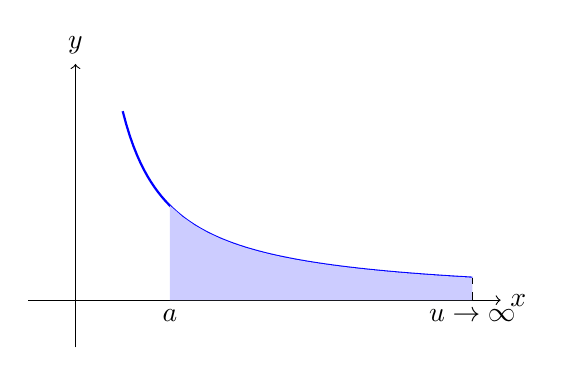
\begin{tikzpicture}[scale=1.2]
    \draw[->] (-0.5,0) -- (4.5,0) node[right] {$x$};
    \draw[->] (0,-0.5) -- (0,2.5) node[above] {$y$};
    \draw[thick, blue, samples=100, domain=0.5:4.2] plot (\x, {1/\x});
    \fill[blue!20, domain=1:4.2] (1,0) -- (1,1) -- plot (\x, {1/\x}) -- (4.2,0) -- cycle;
    \node at (2.5, 0.3) {};
    \draw[dashed] (4.2,0) -- (4.2, {1/4.2});
    \node[below] at (1,0) {$a$};
    \node[below] at (4.2,0) {$u \to \infty$};
\end{tikzpicture}
\caption{Visualizing an integral over an infinite interval}
\end{figure}

Similarly, we can define integrals for other infinite intervals:
\[
\int_{-\infty}^b f(x) dx = \lim_{u \to -\infty} \int_u^b f(x) dx
\]

\[
\int_{-\infty}^{+\infty} f(x) dx = \int_{-\infty}^c f(x) dx + \int_c^{+\infty} f(x) dx
\]

For the integral from $-\infty$ to $+\infty$ to converge, \textbf{both} constituent integrals must converge independently. The choice of the splitting point $c$ does not affect the convergence.
\subsubsection{Benchmark: The $p$-Integral (Type I)}
To determine the convergence of complex functions, we compare them to the power function $1/x^p$.

\begin{theorem}
The integral $\int_1^{+\infty} \frac{1}{x^p} \, dx$:
\begin{itemize}
    \item \textbf{Converges} if $p > 1$.
    \item \textbf{Diverges} if $p \leq 1$.
\end{itemize}
\end{theorem}
\begin{proof}
Evaluating $\int_1^u x^{-p} \, dx$:
\begin{itemize}
    \item If $p=1$, $\ln u \to \infty$ as $u \to \infty$.
    \item If $p \neq 1$, $\frac{u^{1-p}-1}{1-p}$. For convergence, we need $u^{1-p} \to 0$, which requires $1-p < 0 \implies p > 1$.
\end{itemize}
\end{proof}

\subsection{Improper Integrals of the Second Kind (Unbounded Functions)}

These integrals occur on a finite interval $[a,b]$ where the integrand $f(x)$ becomes infinite (has a singularity) at one or more points.

\begin{definition}
If $f$ is continuous on $[a, b)$ and discontinuous at $b$ (e.g., $\lim_{x \to b^-} |f(x)| = \infty$), we define:
\[
\int_a^b f(x) \, dx = \lim_{\epsilon \to 0^+} \int_a^{b-\epsilon} f(x) \, dx
\]
\end{definition}

\subsubsection{Benchmark: The $p$-Integral (Type II)}
Be careful: the convergence condition for singularities is the \textit{reverse} of infinite intervals.

\begin{theorem}
For the interval $(0, 1]$, the integral $\int_0^1 \frac{1}{x^p} \, dx$:
\begin{itemize}
    \item \textbf{Converges} if $p < 1$.
    \item \textbf{Diverges} if $p \geq 1$.
\end{itemize}
\end{theorem}

\subsection{General Theory of Convergence}

Before applying practical tests, we establish the rigorous necessary and sufficient conditions for convergence.

\subsubsection{Cauchy Criterion}
The Cauchy Criterion is fundamental because it allows us to prove convergence without knowing the limit's value.

\begin{theorem}[Cauchy Criterion for Improper Integrals]
The integral $\int_a^{+\infty} f(x) \, dx$ converges \textbf{if and only if} for every $\epsilon > 0$, there exists an $M > a$ such that for all $u_2 > u_1 > M$:
\[
\left| \int_{u_1}^{u_2} f(x) \, dx \right| < \epsilon
\]
\end{theorem}

\subsubsection{Absolute vs. Conditional Convergence}
\begin{itemize}
    \item \textbf{Absolute Convergence:} $\int |f(x)| \, dx$ converges.
    \item \textbf{Conditional Convergence:} $\int f(x) \, dx$ converges, but $\int |f(x)| \, dx$ diverges.
\end{itemize}
\begin{theorem}
If $\int_a^{+\infty} |f(x)| \, dx$ converges, then $\int_a^{+\infty} f(x) \, dx$ converges.
\end{theorem}

\subsection{Convergence Tests}

\subsubsection{Direct Comparison Test}
\begin{theorem}
Let $f(x)$ and $g(x)$ be continuous functions on $[a, +\infty)$ such that $0 \leq f(x) \leq g(x)$ for all $x \geq a$.
\begin{enumerate}
    \item If $\int_a^{+\infty} g(x) dx$ converges, then $\int_a^{+\infty} f(x) dx$ also converges.
    \item If $\int_a^{+\infty} f(x) dx$ diverges, then $\int_a^{+\infty} g(x) dx$ also diverges.
\end{enumerate}
\end{theorem}
\textit{Intuition:} If the area under the larger curve is finite, the area under the smaller curve must be finite. If the area under the smaller curve is infinite, the larger area must be infinite.
\begin{example}

Does $\int_1^{+\infty} \frac{\sin^2 x}{x^2} dx$ converge?
\end{example}
\textbf{Solution:} We know that $0 \leq \sin^2 x \leq 1$. Therefore:
\[
0 \leq \frac{\sin^2 x}{x^2} \leq \frac{1}{x^2}
\]
We know that $\int_1^{+\infty} \frac{1}{x^2} dx$ converges ($p=2 > 1$). By the Direct Comparison Test, $\int_1^{+\infty} \frac{\sin^2 x}{x^2} dx$ converges.
\subsubsection{Limit Comparison Test}

Sometimes finding a direct inequality is difficult. The Limit Comparison Test is often more powerful.

\begin{theorem}
Let $f(x)$ and $g(x)$ be positive continuous functions on $[a, +\infty)$. If:
\[
\lim_{x \to +\infty} \frac{f(x)}{g(x)} = L
\]
where $0 < L < +\infty$, then $\int_a^{+\infty} f(x) dx$ and $\int_a^{+\infty} g(x) dx$ either both converge or both diverge.
\end{theorem}
If $L=0$ and $g(x)$ converges, then $f(x)$ converges. If $L=+\infty$ and $g(x)$ diverges, then $f(x)$ diverges.
\begin{example}
Analyze $\int_1^{+\infty} \frac{x}{1+x^3} dx$.
\end{example}

\textbf{Solution:} For large $x$, the term $1$ is negligible, so $\frac{x}{1+x^3} \approx \frac{x}{x^3} = \frac{1}{x^2}$.

Let $f(x) = \frac{x}{1+x^3}$ and $g(x) = \frac{1}{x^2}$.

\[
\lim_{x \to +\infty} \frac{f(x)}{g(x)} = \lim_{x \to +\infty} \frac{x/(1+x^3)}{1/x^2} = \lim_{x \to +\infty} \frac{x^3}{1+x^3} = 1
\]

Since $L=1$ (finite and positive) and we know $\int_1^{+\infty} \frac{1}{x^2} dx$ converges, the original integral converges.



For positive functions, we use comparison tests. For oscillating functions, we need more advanced tools.

\subsubsection{Cauchy's Limit Comparison Test (Order Analysis)}
This is the most practical method for determining convergence. It formalizes the idea of comparing a function to $1/x^p$.

\begin{theorem}
Let $f(x)$ be a positive function defined on $[a, +\infty)$. Consider the limit of $f(x)$ multiplied by a test power $x^p$:
\[
\lambda = \lim_{x \to +\infty} x^p f(x)
\]
\begin{enumerate}
    \item \textbf{Convergence Case:} If we can find a $p > 1$ such that $0 \le \lambda < +\infty$, then $\int_a^{+\infty} f(x) \, dx$ \textbf{converges}.
    \textit{(Meaning: $f(x)$ goes to zero faster than $1/x$, roughly like $1/x^p$)}
    
    \item \textbf{Divergence Case:} If we can find a $p \le 1$ such that $0 < \lambda \le +\infty$, then $\int_a^{+\infty} f(x) \, dx$ \textbf{diverges}.
    \textit{(Meaning: $f(x)$ goes to zero slower than or equal to $1/x$)}
\end{enumerate}
\end{theorem}

\begin{example}
Test $\int_1^{+\infty} \frac{\ln x}{x^2} \, dx$.
We suspect convergence because $x^2$ dominates. Let's compare with $p=1.5$ (since $1 < 1.5 < 2$, giving us "room").
\[
\lim_{x \to +\infty} x^{1.5} \frac{\ln x}{x^2} = \lim_{x \to +\infty} \frac{\ln x}{x^{0.5}} = 0 \quad (\text{by L'Hopital})
\]
Since $p=1.5 > 1$ and the limit is finite, the integral converges.
\end{example}

\subsubsection{Dirichlet and Abel Tests (For Conditional Convergence)}
These tests are used for integrals of the product form $\int_a^{+\infty} f(x)g(x) \, dx$, typically where one part oscillates and the other decays.

\begin{theorem}[Dirichlet's Test]
The integral $\int_a^{+\infty} f(x)g(x) \, dx$ converges if:
\begin{enumerate}
    \item $f(x)$ has bounded partial integrals: $\exists M, \forall u > a, |\int_a^u f(t) \, dt| \le M$.
    \item $g(x)$ is monotonic decreasing and $\lim_{x \to +\infty} g(x) = 0$.
\end{enumerate}
\end{theorem}
\textit{Classic Application:} $\int_0^{+\infty} \frac{\sin x}{x} \, dx$. Here $f(x)=\sin x$ (bounded integral) and $g(x)=1/x$ (monotonic to 0).

\begin{theorem}[Abel's Test]
The integral $\int_a^{+\infty} f(x)g(x) \, dx$ converges if:
\begin{enumerate}
    \item $\int_a^{+\infty} f(x) \, dx$ converges (the integral itself).
    \item $g(x)$ is monotonic and bounded.
\end{enumerate}
\end{theorem}

\subsubsection{Cauchy Principal Value (P.V.)}

In some divergent integrals, the positive and negative areas might cancel each other out if limits are taken symmetrically. This value is called the Cauchy Principal Value.

\begin{definition}
\begin{enumerate}
    \item For singularities at $c \in (a, b)$:
    \[
    \text{P.V.} \int_a^b f(x) \, dx = \lim_{\epsilon \to 0^+} \left( \int_a^{c-\epsilon} f(x) \, dx + \int_{c+\epsilon}^b f(x) \, dx \right)
    \]
    \item For infinite intervals $(-\infty, +\infty)$:
    \[
    \text{P.V.} \int_{-\infty}^{+\infty} f(x) \, dx = \lim_{R \to +\infty} \int_{-R}^R f(x) \, dx
    \]
\end{enumerate}
\end{definition}

\begin{remark}
\textbf{Convergence $\implies$ P.V. exists}, but the converse is false.
\end{remark}

\begin{example}
Consider $f(x) = \frac{1}{x}$ on $[-1, 1]$.
\begin{itemize}
    \item \textbf{Improper Integral:} $\int_{-1}^1 \frac{1}{x} \, dx = \int_{-1}^0 \frac{1}{x} \, dx + \int_0^1 \frac{1}{x} \, dx$.
    Since $\int_{\epsilon}^1 \frac{1}{x} \, dx = -\ln \epsilon \to \infty$, the standard integral \textbf{diverges}.
    \item \textbf{Principal Value:}
    \[
    \text{P.V.} \int_{-1}^1 \frac{1}{x} \, dx = \lim_{\epsilon \to 0^+} \left( \int_{-1}^{-\epsilon} \frac{1}{x} \, dx + \int_{\epsilon}^1 \frac{1}{x} \, dx \right) = 0
    \]
    (Due to the odd symmetry of the function).
\end{itemize}
\end{example}

\subsubsection{Comprehensive Example: The Gamma Function}
\[
\Gamma(s) = \int_0^{+\infty} x^{s-1} e^{-x} \, dx
\]
This integral requires analysis of both singularity and infinite bounds.
\begin{itemize}
    \item \textbf{At $0$:} If $s < 1$, $x^{s-1}$ has a singularity. Since $e^{-x} \approx 1$, it behaves like $\int_0^1 \frac{1}{x^{1-s}} dx$. By the Type II $p$-test, this converges if $1-s < 1 \implies s > 0$.
    \item \textbf{At $+\infty$:} $e^{-x}$ decays faster than any power $x^p$ grows. Using the Limit Comparison Test with $1/x^2$:
    \[
    \lim_{x \to \infty} x^2 (x^{s-1} e^{-x}) = 0
    \]
    Thus, it converges for all $s$.
\end{itemize}
\textbf{Conclusion:} The integral converges for $s > 0$.

At the end of this chapter, let's use the knowledge we learned to solve an interesting problem: the Gabriel's Horn.

Considering we have a horn, whose cross section is a circle but longitudinal section is function $y = \frac{1}{x}, x \in (1,\infty)$.

Let's first calculate the volume of the horn:

\[V = \pi \int_{1}^{+\infty} (\frac{1}{x})^2 dx = \pi [-\frac{1}{x}]_{1}^{+\infty} = \pi\]

We can see that the horn have finite volume.

Then calculate the surface area of the horn.

\[
S = 2\pi \int_{1}^{+\infty} \frac{1}{x} \sqrt{1+\frac{1}{x^4}} dx \geq 2\pi \int_{1}^{+\infty} \frac{1}{x} dx = +\infty
\]

The integration product of the surface area is divergent.

Here comes a very interesting paradox. We can use finite many paint to fill the horn, but this horn of paint cannot coated the inner wall of the horn.

This consequence is contradicting to our naive understanding.

As we close this chapter, remember that this is not an end, but a gateway. The journey of mathematical analysis continues: in the \textbf{Chapter 4}, we will extend these foundations to higher dimensions, study curves and surfaces in greater depth, and encounter even more beautiful and unexpected results. The horn's call, echoing from the realm of the infinite, invites us to explore further.

In later chapters, we will move on to more advanced topics in analysis, such as multi-variables calculus, differential equations, complex analysis and functional analysis. Each of these areas builds upon the concepts we have developed here, and each offers its own unique insights and challenges. We encourage readers to continue their exploration, armed with the rigorous tools and deep understanding gained from this chapter.


\vspace{1cm}
\noindent
\textbf{References:} \\
Mathematical Analysis (Third Edition), Chen, J., Higher Education Press \\
The Real Numbers and Real Analysis, Ethan D. Bloch, Springer


